\documentclass[11pt]{article}
\usepackage[T1]{fontenc}
\usepackage[utf8]{inputenc}
\usepackage{lmodern}
\usepackage[margin=1.08in]{geometry}
\usepackage{amsmath,amssymb,amsthm,mathtools,bm}
\usepackage{microtype}
\usepackage{graphicx,booktabs,tabularx,array,float,caption}
\usepackage{setspace}
\usepackage[round,authoryear]{natbib}
\usepackage{xcolor}
\usepackage{enumitem}
\usepackage[section]{placeins}
\usepackage[hidelinks]{hyperref}
\hypersetup{pdftitle={The Mathematics of Generative Neural Operators},
 pdfauthor={Miquel Noguer i Alonso},
 pdfsubject={DOI: 10.5281/zenodo.22714854}}
\usepackage[nameinlink,noabbrev]{cleveref}
\numberwithin{equation}{section}
\newtheorem{theorem}{Theorem}[section]
\newtheorem{proposition}[theorem]{Proposition}
\newtheorem{lemma}[theorem]{Lemma}
\newtheorem{corollary}[theorem]{Corollary}
\theoremstyle{definition}
\newtheorem{definition}[theorem]{Definition}
\newtheorem{assumption}[theorem]{Assumption}
\crefname{assumption}{assumption}{assumptions}
\Crefname{assumption}{Assumption}{Assumptions}
\newtheorem{example}[theorem]{Example}
\theoremstyle{remark}
\newtheorem{remark}[theorem]{Remark}
\newcommand{\E}{\mathbb E}
\newcommand{\R}{\mathbb R}
\newcommand{\N}{\mathbb N}
\newcommand{\Law}{\operatorname{Law}}
\newcommand{\tr}{\operatorname{tr}}
\newcommand{\Id}{\operatorname{Id}}
\newcommand{\Ran}{\operatorname{Ran}}
\newcommand{\Lip}{\operatorname{Lip}}
\newcommand{\Ptwo}{\mathcal P_2}
\newcommand{\dd}{\,\mathrm d}
\newcommand{\norm}[1]{\left\lVert#1\right\rVert}
\newcommand{\ip}[2]{\left\langle#1,#2\right\rangle}
\newcommand{\push}{_{\#}}
\newcommand{\eps}{\varepsilon}
\setlength{\emergencystretch}{2em}
\setstretch{1.08}
\captionsetup{font=small,labelfont=bf}
\setlength{\parindent}{1.25em}
\setlength{\parskip}{0pt}
\pagestyle{empty}
\setlist[itemize]{leftmargin=1.5em,itemsep=0.2em,topsep=0.35em}
\allowdisplaybreaks[1]
\title{\textbf{The Mathematics of Generative Neural Operators}\\[0.35em]
\large Resolution Consistency, Conditional Refinement,\\ and Hidden-State Obstructions}
\author{Miquel Noguer i Alonso\\
\small Artificial Intelligence Finance Institute (AIFI)}
\date{\today}
\begin{document}
\maketitle
\thispagestyle{empty}
\begin{center}\small\href{https://doi.org/10.5281/zenodo.22714854}{DOI: 10.5281/zenodo.22714854}\end{center}
\begin{abstract}
Generative neural operators learn laws on function spaces, but resolution convergence, agreement of projected samples, and autonomous coarse dynamics impose distinct requirements. We connect these requirements to quantitative approximation and statistical guarantees. For a prescribed interpolation, a conditional-variance identity gives the exact population loss of coarse autonomy; a Gaussian commutation criterion and transport-cost calculation make the obstruction explicit. Conditional refinement instead preserves previously sampled coordinates. Its error satisfies a sharp orthogonal recurrence whose exact energy gain yields a necessary and sufficient squared-sensitivity condition for class-uniform robustness. Under summable fitting errors, the construction defines a genuine Hilbert-valued law. An exact transport decomposition separates unresolved energy, while minimax and kernel-factorization results delimit identifiability and autonomous simulation in physical time. Riesz coordinates and bi-Lipschitz decoders extend the metric comparison beyond orthogonal physical observations. A dependency-sensitive certificate retains the actual architecture's coordinate dependence and avoids unnecessary error propagation. Conditional flow-matching losses and globally bounded spectral networks provide concrete certificate inputs. For bounded scalar details, an independent two-split audit estimates conditional-law error from observed fields without evaluating the target conditional mean. Its simultaneous event covers candidate and resolution selection, subject to explicit support, sufficient-context, regularity, and tail assumptions. Three-seed neural experiments distinguish this certificate from measured coupling error and quantify the cost of statistical uncertainty. A Lean project checks 35 declarations, including finite probabilistic refinement, the exact two-dimensional spectral bound and its attainment, dependency propagation, and observation distortion. The remaining measure-theoretic and statistical arguments are supplied as written proofs with explicit formalization boundaries.
\end{abstract}
\noindent\textbf{Keywords:} generative neural operators; conditional transport; flow matching; projective consistency; Wasserstein distance; hidden state; multiresolution analysis.
\clearpage
\setcounter{tocdepth}{2}
\tableofcontents
\clearpage
\section{Introduction}
A generative model of a random field should describe one probabilistic object across the resolutions at which that object is observed. A simulator of an order book, for example, may produce liquidity aggregated over price intervals, liquidity at individual prices, and latent reserve quantities. A model of a physical field may produce low Fourier modes and their unresolved fluctuations. In both cases, fitting a collection of finite arrays leaves open whether those arrays belong to a common law and whether the dynamics used to generate them respect the chosen observation hierarchy.

Neural operators provide architectures for approximating maps between function spaces \citep{kovachki2023}. Their generative counterparts learn a pushforward law rather than a single solution operator. Generative adversarial neural operators make this construction explicit \citep{rahman2022}. Diffusion and flow formulations extend the available transports to function-valued random objects \citep{pidstrigach2025,lim2025,kerrigan2024functional}. These developments establish the basic modeling language. The present paper studies a compatibility problem within that language: how should a generative transport respond to the removal or addition of observable coordinates?

Four notions must be distinguished. \emph{Discretization convergence} asks whether increasingly accurate numerical realizations approach a continuum operator. \emph{Projective consistency} asks whether the projected fine law equals the coarse law. \emph{Pathwise consistency} strengthens this to equality of projected samples under a specified coupling, such as shared coarse randomness. \emph{Autonomous projected dynamics} asks whether the velocity or transition law of the coarse state is determined by that state alone. Autonomous projected dynamics can fail even when a continuum model exists and every coarse marginal is known exactly.

Our starting point is an information identity. For a full velocity $v_s(X_s)$ and an orthogonal observation $P$, the best coarse-only approximation to $Pv_s(X_s)$ is its conditional expectation given $PX_s$. The remaining conditional variance is an irreducible population error. We apply this identity to a prescribed generative bridge, evaluate it exactly for correlated Gaussian targets, and show why projecting the optimal velocity can change the generated endpoint law. The obstruction concerns the specified bridge and the chosen information restriction; it does not rule out other transports with the same target law.

The constructive result uses conditional refinement. After generating a coarse sample, the model holds it fixed and samples the next orthogonal detail band conditional on it. This is a resolution hierarchy of conditional transports. If $\eps_j$ is the conditional distribution error at level $j$, $L_j$ is the sensitivity of the learned detail law to its input context, and $d_j$ is a propagated error bound, then
\begin{equation}\label{eq:intro-recurrence}
 d_j^2=d_{j-1}^2+(\eps_j+L_jd_{j-1})^2,
 \qquad d_{-1}=0.
\end{equation}
The recurrence is sharp in the kernel class considered here. We also compute its exact worst-case amplification of aggregate fitting energy through a two-dimensional eigenvalue recursion. This gives a necessary and sufficient squared-sensitivity condition for uniform robustness over the full conditional-kernel class. Orthogonality also yields the exact decomposition
\begin{equation}\label{eq:intro-tail}
 W_2^2(\mu,\widehat\mu_m)
 =\E\norm{(I-P_m)U}^2+W_2^2((P_m)\push\mu,\widehat\mu_m)
\end{equation}
when $\widehat\mu_m$ is supported on the retained subspace. Consequently, conditional fitting errors and unresolved tail energy enter through different mathematical mechanisms.

The results extend beyond a fixed truncation. If $\sum_j\eps_j^2<\infty$ and $\sum_jL_j^2<\infty$, the refinement construction defines a genuine Hilbert-valued random element, with an explicit Wasserstein bound independent of the terminal level. Conditional flow-matching excess losses provide the $\eps_j$ through a one-sided ODE stability estimate. This connects a population training objective to both the existence and the accuracy of the function-space law.

The same framework separates geometry, architecture, and statistical information. Stable Riesz coordinates or a bi-Lipschitz decoder transfer coefficient certificates to nonorthogonal physical representations. A coordinatewise dependency bound can improve on the class-uniform recurrence when later kernels ignore inaccurate earlier coordinates. Finally, an observed-sample audit controls scalar conditional laws through empirical transport in feature cells and an independent aggregation split. It removes the need to evaluate a target conditional mean, while exposing the sufficient-context and regularity assumptions that make conditional estimation possible. An unseen-cell lower bound explains why these assumptions cannot be omitted.

\subsection{Relation to established transport and operator theory}
The construction of function-space neural operators and their approximation properties is developed by \citet{kovachki2023}. Continuum attention provides a corresponding operator interpretation of transformer layers \citep{calvello2024}. Flow matching and stochastic interpolants identify velocity fields by regression on prescribed probability paths \citep{lipman2023,albergo2023}. Functional flow matching extends that viewpoint to infinite-dimensional laws \citep{kerrigan2024functional}. Valid reference measures and endpoint regularity remain substantive assumptions; trace-class noise alone does not settle the regularity of the sampling equation. \citet{chen2026} study how spectral noise and interpolation schedules affect these issues.

Conditional transport is also established. \citet{hosseini2025} develop triangular optimal transport on separable function spaces. \citet{kerrigan2024conditional} give a dynamical formulation and simulation-free conditional flows. \citet{chemseddine2025} study conditional Wasserstein distances and their relevance for learning conditional laws. Our conditional kernel discrepancy is an instance of this geometry. Triangular Gaussian cost comparisons and adapted Gaussian transport are treated by \citet{bukin2018,acciaio2025}. We use standard disintegration and kernel randomization \citep{kallenberg2021}; we do not claim a new existence theorem for conditional transport itself.

The contribution is the connection between a prescribed-bridge autonomy defect, a sharp orthogonal error recurrence for an entire resolution hierarchy, and a summability criterion that converts conditional fitting guarantees into a coherent function-space law. The finite-dimensional Gaussian commutation criterion makes the obstruction explicit. A companion Gaussian result computes the exact transport-cost premium of resolution autonomy and constructs an autonomous bridge attaining it. The observation minimax result and physical-time kernel criterion delimit what the resulting law can identify and what an autonomous simulator can preserve. Each statement is proved under explicit assumptions. The numerical section tests these statements and trains a shared spectral neural generator on noisy field coefficients. An architecture theorem provides its global sensitivity and energy bounds, and an independent conditional audit supplies simultaneous finite-sample law certificates. The controlled experiment establishes performance within its stated synthetic model.

The closest perturbation antecedents include \citet{rudolf2018}, who control the effect of one-step kernel errors under Wasserstein stability and ergodicity assumptions. Our hierarchy is not an ergodic chain on a fixed state space: it retains the entire previous state and appends an orthogonal coordinate. The resulting improvement is displayed in \Cref{sec:comparison}. \citet{irons2022} establish statistical consistency and rates for triangular-flow estimators under smoothness assumptions. Their estimator theory and our conditional validation certificate address different tasks; the latter certifies a fixed trained hierarchy using an independent audit, without asserting an optimization rate.

\subsection{Organization}
\Cref{sec:setting} fixes the probabilistic and geometric setting. \Cref{sec:obstruction} derives the autonomy defect. \Cref{sec:refinement,sec:certificate} construct conditional refinement and prove the main error and existence results. \Cref{sec:fm} links the certificate to flow matching. \Cref{sec:information} treats observation limits and physical time. \Cref{sec:riesz} treats nonorthogonal and nonlinear representations. \Cref{sec:architecture,sec:observed-audit} give implemented stability, observed-data auditing, and dependency-sensitive propagation. \Cref{sec:experiments,sec:application} report numerical evidence and a market-modeling application.

\section{Function-space laws and resolution hierarchies}\label{sec:setting}
Let $H$ be a real separable Hilbert space with norm $\norm{\cdot}$ and let $\Ptwo(H)$ denote its Borel probability measures with finite second moment. For $\alpha,\beta\in\Ptwo(H)$, define
\begin{equation}
 W_2^2(\alpha,\beta)=\inf_{\pi\in\Pi(\alpha,\beta)}
 \int_{H\times H}\norm{u-v}^2\,\pi(\mathrm du,\mathrm dv).
\end{equation}
A condition $c$ in a standard Borel space specifies a target kernel $c\mapsto\mu_c$. Unless stated otherwise, all arguments fix $c$ and suppress it. This avoids confusing external conditioning with conditioning on previously generated resolution bands. For jointly measurable kernels the constructions can include $c$ throughout; uniform or integrated conclusions require the corresponding constants to be uniform or integrable in $c$.

\begin{definition}[Generative operator]
A measurable map $G:C\times Z\to H$, together with a reference probability measure $\nu$ on a standard Borel latent space $Z$, defines the conditional generated law $G(c,\cdot)\push\nu$. A neural operator is a parameterized implementation of such a map, or of the conditional velocities used to construct it.
\end{definition}
Measurable representability, continuous operator approximation, statistical learnability, and numerical approximation are separate properties. In particular, a measurable representation theorem below will not assert approximation by a fixed finite neural architecture.

Fix finite-rank orthogonal projections
\begin{equation}\label{eq:hierarchy}
 P_{-1}=0,\qquad P_jP_k=P_{\min(j,k)},\qquad P_j\to I\quad\text{strongly}.
\end{equation}
Write $H_j=\Ran P_j$, $\Delta_j=P_j-P_{j-1}$, and $E_j=\Ran\Delta_j$. Then
\begin{equation}
 H=\overline{\bigoplus_{j\ge0}E_j},\qquad
 X_j=P_jU,\quad B_j=\Delta_jU,\quad U\sim\mu.
\end{equation}
Let $\mu_j=(P_j)\push\mu$, regarded as a law on $H_j$ or embedded in $H$. Fourier bands, wavelet detail spaces, and nested Galerkin spaces fit this setting. Nested observations on irregular grids require a specified inner product and compatible orthogonal reconstruction. Arbitrary point subsampling is not automatically an orthogonal projection.

\begin{definition}[Projective and pathwise consistency]\label{def:consistency}
A family $\{\widehat\mu_j\}$ is projectively consistent if $(P_j)\push\widehat\mu_k=\widehat\mu_j$ for $j\le k$. A coupled family $\{\widehat X_j\}$ is pathwise consistent if $P_j\widehat X_k=\widehat X_j$ almost surely for $j\le k$. A family of numerical generators is discretization convergent if its reconstructed outputs converge to a specified continuum generator in the stated topology.
\end{definition}
Pathwise consistency implies projective consistency. Discretization convergence alone does not require exact equality at any pair of finite resolutions. Likewise, a consistent collection of finite laws need not be supported by $H$ without an energy condition. Independent unit-variance coordinates, for example, give consistent finite Gaussian laws but have infinite squared $\ell^2$ norm almost surely.

\subsection{Reference noise and observation geometry}
An $H$-valued centered Gaussian reference has a positive self-adjoint trace-class covariance $C$:
\begin{equation}\label{eq:gaussian-noise}
 Z=\sum_{k\ge1}\sqrt{\lambda_k}\,\xi_ke_k,
 \qquad \sum_{k\ge1}\lambda_k<\infty,
 \qquad \E\norm Z^2=\tr C.
\end{equation}
Here $\xi_k$ are independent standard normals and $(e_k)$ is an orthonormal eigenbasis. There is no $H$-valued $\mathcal N(0,I)$ in infinite dimension. Function-space diffusion theory treats this issue directly \citep{pidstrigach2025,lim2025}. In the refinement construction each individual $E_j$ is finite dimensional, so standard Gaussian band noise is legitimate; the existence of the infinite output is proved separately.

The chosen norm specifies the accuracy claim. For $H=L^2(D)$, the error measures integrated field discrepancy and allows discontinuous fields. Point values are not well-defined on $L^2$ equivalence classes. Cell averages and bounded linear functionals are valid observations; point evaluation requires a stronger state space. A Sobolev norm can emphasize derivatives, but only for target laws having the required second moment. Changing the norm changes both the tail energy and the constants in the results below.

\section{The information cost of autonomous coarse dynamics}\label{sec:obstruction}
Let $(Z,U)$ have any coupling of a reference law and a target law in $\Ptwo(H)$. For the straight interpolation
\begin{equation}\label{eq:global-bridge}
 X_s=(1-s)Z+sU,\qquad V=U-Z,\qquad 0\le s\le1,
\end{equation}
define $v_s^\star(X_s)=\E[V\mid X_s]$. Conditional expectations are understood in the Hilbert-valued $L^2$ sense, jointly with the time variable. The population flow-matching loss is
\begin{equation}\label{eq:global-loss}
 \mathcal L(v)=\int_0^1\E\norm{v_s(X_s)-V}^2\dd s.
\end{equation}
Fix an orthogonal projection $P$ and let $Q=I-P$. A velocity is \emph{coarse-autonomous} if $Pv_s(x)=b_s(Px)$ for a measurable $PH$-valued function $b_s$. This is a restriction on available information, independent of the number of model parameters.

\begin{theorem}[Exact autonomy defect]\label{thm:defect}
Define
\begin{align}
 \bar v_s(PX_s)&=\E[Pv_s^\star(X_s)\mid PX_s]=\E[PV\mid PX_s],\\
 D_P(s)&=\E\norm{Pv_s^\star(X_s)-\bar v_s(PX_s)}^2,
 \qquad \mathfrak D_P=\int_0^1D_P(s)\dd s.
\end{align}
For every square-integrable coarse-autonomous velocity $v$,
\begin{align}\label{eq:defect-decomposition}
 \mathcal L(v)-\mathcal L(v^\star)
 =\mathfrak D_P
 &+\int_0^1\E\norm{b_s(PX_s)-\bar v_s(PX_s)}^2\dd s\notag\\
 &+\int_0^1\E\norm{Q(v_s(X_s)-v_s^\star(X_s))}^2\dd s.
\end{align}
Thus $\mathfrak D_P$ is the exact excess-loss infimum over this measurable velocity class. It vanishes if and only if $Pv_s^\star(X_s)$ is measurable with respect to $PX_s$ for almost every $s$, up to the relevant null sets.
\end{theorem}
\begin{proof}
Conditional-expectation orthogonality first gives
\[
 \mathcal L(v)-\mathcal L(v^\star)
 =\int_0^1\E\norm{v_s(X_s)-v_s^\star(X_s)}^2\dd s.
\]
Split the squared norm into orthogonal $P$ and $Q$ components. In the $P$ component insert $\bar v_s(PX_s)$. The cross term vanishes because $b_s(PX_s)-\bar v_s(PX_s)$ is $PX_s$-measurable and the remaining difference has conditional mean zero. This proves \eqref{eq:defect-decomposition}. The measurable choice $v_s(x)=\bar v_s(Px)+Qv_s^\star(x)$ attains the infimum. The final equivalence is the zero-residual characterization of conditional expectation.
\end{proof}

The minimizing measurable velocity need not generate a well-posed ODE. Consequently, the theorem is an exact regression statement and a lower bound for any regular neural subclass, rather than an unconditional flow-existence result. Moreover, a positive $\mathfrak D_P$ need not lower-bound the endpoint Wasserstein error: another velocity can reach the same endpoint along a different probability path.

\begin{proposition}[A hierarchy of information restrictions]\label{prop:hierarchy-defect}
For a finite hierarchy through level $m$, impose
$\Delta_jv_s(x)=b_{j,s}(P_jx)$ for every $0\le j\le m$, on $H_m$. The exact excess-loss infimum equals
\begin{equation}\label{eq:hierarchy-defect}
 \sum_{j=0}^m\int_0^1\E\norm{
 \Delta_jv_s^\star(X_s)-\E[\Delta_jv_s^\star(X_s)\mid P_jX_s]}^2\dd s.
\end{equation}
If the information used for one band is enlarged from a sigma-field $\mathcal G_1$ to $\mathcal G_2\supseteq\mathcal G_1$, its defect decreases by
\begin{equation}
 \int_0^1\E\norm{\E[\Delta_jv_s^\star(X_s)\mid\mathcal G_2]
 -\E[\Delta_jv_s^\star(X_s)\mid\mathcal G_1]}^2\dd s.
\end{equation}
\end{proposition}
\begin{proof}
Apply Hilbert-space conditional-expectation orthogonality separately to the mutually orthogonal bands. The second identity follows by the tower property and the same orthogonality argument for nested information sets.
\end{proof}
The proposition quantifies the value of a retained hidden-state summary for velocity prediction. Zero defect for this particular velocity is weaker than sufficiency for all conditional observables of the endpoint law.

\subsection{Gaussian bridges: an exact commutation criterion}
We now work in $\R^d$; the spherical Gaussian reference in this subsection is finite dimensional. Let $Z\sim\mathcal N(0,I)$ and $U\sim\mathcal N(0,\Sigma)$ be independent, with $\Sigma$ positive definite. Set
\begin{equation}\label{eq:gaussian-velocity}
 C_s=(1-s)^2I+s^2\Sigma,\qquad
 A_s=(s\Sigma-(1-s)I)C_s^{-1}.
\end{equation}
Gaussian regression gives $v_s^\star(x)=A_sx$.

\begin{theorem}[Covariance commutation and autonomous Gaussian bridges]\label{thm:gaussian-commutation}
For any orthogonal projection $P$ and any $0<s<1$,
\begin{equation}\label{eq:gaussian-defect}
 D_P(s)=\tr\left(PA_sQ\,C_{Q\mid P,s}\,QA_s^TP\right),
\end{equation}
where, as an operator on $Q\R^d$,
\begin{equation}
 C_{Q\mid P,s}=QC_sQ-QC_sP(PC_sP|_{P\R^d})^{-1}PC_sQ.
\end{equation}
The following conditions are equivalent:
\begin{enumerate}[label=(\roman*)]
\item $D_P(s)=0$ for one $s\in(0,1)$;
\item $D_P(s)=0$ for every $s\in(0,1)$;
\item $P\Sigma=\Sigma P$.
\end{enumerate}
\end{theorem}
\begin{proof}
Conditional on $PX_s$, the residual fine coordinate is centered Gaussian with covariance $C_{Q\mid P,s}$. The unpredicted coarse velocity is $PA_sQ(X_s-\E[X_s\mid PX_s])$, giving \eqref{eq:gaussian-defect}. The Schur complement $C_{Q\mid P,s}$ is positive definite on $Q\R^d$, so the defect is zero exactly when $PA_sQ=0$. Since $A_s$ is symmetric, this is equivalent to $P$ commuting with $A_s$. For $0<s<1$,
\begin{equation}
 A_s=\frac1sI-\frac{1-s}{s}C_s^{-1}.
\end{equation}
Commutation with $A_s$ is therefore equivalent to commutation with $C_s$, and hence with $\Sigma$. This also proves independence of the chosen interior time.
\end{proof}

\begin{example}[Two correlated coordinates]\label{ex:gaussian}
Let $P(x_1,x_2)=(x_1,0)$ and
\begin{equation}
 \Sigma=\begin{pmatrix}1&\rho\\\rho&1\end{pmatrix},\qquad |\rho|<1,
 \qquad a_s=(1-s)^2+s^2.
\end{equation}
The off-diagonal velocity coefficient and its information defect are
\begin{align}\label{eq:rho-defect}
 (A_s)_{12}&=\frac{\rho s(1-s)}{a_s^2-s^4\rho^2},\\
 D_P(s)&=\frac{\rho^2s^2(1-s)^2}{a_s(a_s^2-s^4\rho^2)},
 \qquad D_P(1/2)=\frac{2\rho^2}{4-\rho^2}.
\end{align}
For $\rho=0.8$, the midpoint defect is $8/21\simeq0.380952$. The best coarse velocity is $\bar v_{1,s}(x_1)=(2s-1)x_1/a_s$. Replacing the first row of $A_s$ by this coarse-only row attains the restricted population loss infimum, but its joint endpoint covariance differs from $\Sigma$; \Cref{sec:experiments} evaluates the discrepancy.
\end{example}

\subsection{Marginal evolution and pathwise closure}
For a smooth bounded cylindrical test function $\varphi$ on $PH$, the bridge satisfies
\begin{equation}
 \frac{\mathrm d}{\mathrm ds}\E\varphi(PX_s)
 =\E\ip{D\varphi(PX_s)}{PV}
 =\E\ip{D\varphi(PX_s)}{\bar v_s(PX_s)}.
\end{equation}
Thus $\bar v_s$ gives the weak continuity equation for the coarse marginals. When its ODE and continuity equation are well posed, it generates those marginals. It does not in general reproduce the projection of individual full-flow trajectories, or the joint law with the fine coordinates. The information defect is precisely the regression obstruction to that stronger closure of the prescribed velocity field.

\section{Conditional refinement with exact projection consistency}\label{sec:refinement}
The previous obstruction suggests changing the transport construction. Generate a coarse endpoint first and then sample the missing detail conditional on that endpoint. At level $j$, disintegrate the target law as
\begin{equation}\label{eq:target-kernel}
 K_j(x,\cdot)=\Law(B_j\mid X_{j-1}=x),\qquad x\in H_{j-1}.
\end{equation}
For $j=0$, the context is $X_{-1}=0$ and $K_0(0,\cdot)=\mu_0$. Versions outside the target context support may be defined arbitrarily. Learned kernels below are specified for every context that the learned model can visit.

\begin{theorem}[Coherent conditional representation]\label{thm:representation}
For every $\mu\in\Ptwo(H)$ and hierarchy \eqref{eq:hierarchy}, there are measurable maps $T_j:H_{j-1}\times(0,1)\to E_j$ such that, with independent uniform random variables $\xi_j$,
\begin{equation}\label{eq:tower}
 X_{-1}=0,\qquad B_j=T_j(X_{j-1},\xi_j),\qquad X_j=X_{j-1}+B_j,
\end{equation}
has law $\mu_j$ at every level and is pathwise consistent. The series $\sum_{j\ge0}B_j$ converges almost surely in $H$ and in $L^2(\Omega;H)$ to $U^\dagger\sim\mu$.

For arbitrary measurable learned maps $\widehat T_j$ taking values in $E_j$, the analogous recursion is pathwise consistent at every finite level. If
\begin{equation}\label{eq:learned-energy}
 \sup_m\E\norm{\widehat X_m}^2<\infty,
\end{equation}
then it also defines a unique limiting law $\widehat\mu\in\Ptwo(H)$ whose projections are the generated finite-level laws.
\end{theorem}
\begin{proof}
The spaces involved are standard Borel. Disintegration gives the kernels $K_j$, and kernel randomization gives maps $T_j$ with $(T_j(x,\cdot))\push\mathrm{Unif}(0,1)=K_j(x,\cdot)$; these standard constructions are treated in \citet{kallenberg2021}. Induction using \eqref{eq:target-kernel} proves $\Law(X_j)=\mu_j$. Because $B_j\in E_j$, $P_kX_j=X_k$ for $k\le j$. Orthogonality gives
\[
 \E\sum_{j\ge0}\norm{B_j}^2
 =\lim_m\E\norm{P_mU}^2=\E\norm U^2<\infty.
\]
Thus the nonnegative series is finite almost surely, which makes the orthogonal vector series converge in $H$. Its mean-square tail also tends to zero. The limit has all projected laws $\mu_j$; the coordinate sigma-field of a complete countable orthonormal basis generates the Borel sigma-field of $H$, so its law is $\mu$.

For learned maps the same pathwise identity holds algebraically. Under \eqref{eq:learned-energy}, monotone convergence gives $\E\sum_j\norm{\widehat B_j}^2<\infty$. The same argument proves almost-sure and mean-square convergence, and uniqueness follows from the projected laws.
\end{proof}

The representation is measure theoretic. It includes singular and discrete conditional laws and does not imply that their maps are continuous. A regular ODE implementation requires the additional assumptions in \Cref{sec:fm}. Independent uniforms can be replaced by non-atomic finite-dimensional band references via measurable randomization; no infinite identity-covariance Gaussian is introduced by this representation.

\subsection{Conditional flows within the detail fibers}
For a fixed coarse state $x\in H_{j-1}$, choose $Z_j\sim\nu_j\in\Ptwo(E_j)$ and $B_j^x\sim K_j(x,\cdot)$ independently, and define
\begin{equation}\label{eq:conditional-bridge}
 I^x_{j,r}=(1-r)Z_j+rB_j^x,\qquad
 w_j^\star(r,z;x)=\E[B_j^x-Z_j\mid I^x_{j,r}=z],\quad 0\le r\le1.
\end{equation}
The coarse component $x$ stays fixed. A learned detail flow solves
\begin{equation}\label{eq:detail-ode}
 \dot Y_r=\widehat w_j(r,Y_r;x),\qquad Y_0=Z_j,
 \qquad \widehat T_j(x,Z_j)=Y_1.
\end{equation}
Each refinement alters only $E_j$, so numerical integration errors within $E_j$ do not change earlier bands. The construction is a sequence of conditional transports of the type studied in \citet{hosseini2025,kerrigan2024conditional}; its use here is to control an entire orthogonal hierarchy.

For \Cref{ex:gaussian}, first sample $X_1\sim\mathcal N(0,1)$ and then sample $X_2\mid X_1=x\sim\mathcal N(\rho x,1-\rho^2)$. Put $\sigma^2=1-\rho^2$. The conditional interpolation in \eqref{eq:conditional-bridge} has velocity
\begin{equation}\label{eq:conditional-gaussian-velocity}
 w^\star(r,y;x)=\rho x+
 \frac{r\sigma^2-(1-r)}{(1-r)^2+r^2\sigma^2}(y-r\rho x).
\end{equation}
Its flow map is
\begin{equation}\label{eq:conditional-gaussian-map}
 \Phi_r(z;x)=r\rho x+\sqrt{(1-r)^2+r^2\sigma^2}\,z.
\end{equation}
Differentiation verifies \eqref{eq:conditional-gaussian-velocity}; at $r=1$, $\Phi_1(z;x)=\rho x+\sigma z$. Thus the target correlation is reproduced exactly while the coarse endpoint is unchanged. This flow uses a different probability path from the global straight bridge of \Cref{ex:gaussian}.

\subsection{The exact transport cost of Gaussian resolution autonomy}
The ability to reach a target law does not mean that a resolution-preserving transport has the same cost as an unrestricted one. Triangular Gaussian transport costs and their comparison with unrestricted costs have been studied by \citet{bukin2018}, while \citet{acciaio2025} give Gaussian adapted-transport formulas. The following specialization uses the classical triangular structure \citep{rosenblatt1952,hosseini2025} to connect the resolution order to an explicit autonomous flow and its action. The Gaussian cost comparison itself is established transport geometry.

Work in $\R^d=\bigoplus_{j=0}^mE_j$. Let $Z\sim\mathcal N(0,I)$ and $U\sim\mathcal N(0,\Sigma)$, with $\Sigma>0$. Write $U_{<j}=(U_0,\ldots,U_{j-1})$ and let
\begin{equation}\label{eq:schur-bands}
 M_j=\Sigma_{j,<j}\Sigma_{<j,<j}^{-1},\qquad
 S_j=\Sigma_{jj}-\Sigma_{j,<j}\Sigma_{<j,<j}^{-1}\Sigma_{<j,j}.
\end{equation}
At the first band, $M_0U_{<0}=0$ and $S_0=\Sigma_{00}$. A map is \emph{resolution triangular} if its $j$th output band depends only on $(Z_0,\ldots,Z_j)$.

\begin{theorem}[Gaussian transport premium for resolution autonomy]\label{thm:price}
Among all measurable resolution-triangular maps $T$ satisfying $T\push\mathcal N(0,I)=\mathcal N(0,\Sigma)$, the minimum quadratic displacement cost is
\begin{equation}\label{eq:triangular-cost}
 J_{\mathrm{tri}}=\tr\Sigma+d-2\sum_{j=0}^m\tr(S_j^{1/2}).
\end{equation}
It is attained by the linear triangular recursion
\begin{equation}\label{eq:gaussian-triangular-map}
 U_j=M_jU_{<j}+S_j^{1/2}Z_j,\qquad U=LZ.
\end{equation}
The excess over the unrestricted optimal transport cost is
\begin{equation}\label{eq:transport-premium}
 J_{\mathrm{tri}}-W_2^2(\mathcal N(0,I),\mathcal N(0,\Sigma))
 =2\left[\tr(\Sigma^{1/2})-\sum_{j=0}^m\tr(S_j^{1/2})\right]\ge0.
\end{equation}
The excess is zero if and only if $\Sigma$ is block diagonal in the resolution decomposition.

Moreover, $J_{\mathrm{tri}}$ is the minimum kinetic action
$\int_0^1\E\norm{\dot\Phi_s(Z)}^2\dd s$ among absolutely continuous triangular deterministic paths with $\Phi_0=I$ and the prescribed Gaussian terminal law. It is attained by $\Phi_s=(1-s)I+sL$, whose velocity is
\begin{equation}\label{eq:autonomous-gaussian-flow}
 v_s(x)=(L-I)((1-s)I+sL)^{-1}x.
\end{equation}
Every projected velocity in this construction is autonomous.
\end{theorem}
\begin{proof}
For any triangular map, $U_{<j}$ is a function of $Z_{<j}$, so $Z_j$ remains standard Gaussian conditional on $U_{<j}$. The required target conditional law of $U_j$ is $\mathcal N(M_jU_{<j},S_j)$. The Gaussian transport formula gives
\[
 \E[\norm{U_j-Z_j}^2\mid U_{<j}]
 \ge\norm{M_jU_{<j}}^2+\tr S_j+\dim E_j-2\tr S_j^{1/2}.
\]
Summing expectations yields \eqref{eq:triangular-cost}. Recursion \eqref{eq:gaussian-triangular-map} has the required conditional distributions and attains equality band by band.

The unrestricted Gaussian formula gives the difference in \eqref{eq:transport-premium}. To establish its equality condition without a uniqueness assumption, observe that every coupling of $Z$ and $U$ satisfies
\begin{align}
 &\E\norm{U-Z}^2-
   W_2^2(\mathcal N(0,I),\mathcal N(0,\Sigma))\notag\\
 &\hspace{8mm}=\E\left[(U-\Sigma^{1/2}Z)^T\Sigma^{-1/2}
                              (U-\Sigma^{1/2}Z)\right].
\end{align}
Thus equality forces $U=\Sigma^{1/2}Z$ almost surely. If the triangular optimizer has this property, the matrix $\Sigma^{1/2}$ must be block lower triangular, since $Z$ has full support. It is symmetric, hence block diagonal, and so is $\Sigma$. Conversely, block diagonal $\Sigma$ plainly attains zero excess.

For every absolutely continuous sample path, Cauchy--Schwarz gives
$\norm{\Phi_1(Z)-Z}^2\le\int_0^1\norm{\dot\Phi_s(Z)}^2\dd s$.
Its triangular endpoint has cost at least $J_{\mathrm{tri}}$. The straight map path generated by $L$ attains equality. Its diagonal blocks $(1-s)I+sS_j^{1/2}$ are positive definite, so the inverse exists for every $s\in[0,1]$ and is block lower triangular. Formula \eqref{eq:autonomous-gaussian-flow} follows, and its first $j$ output bands depend only on the first $j$ input bands.
\end{proof}

In two dimensions with correlation $\rho$,
\begin{align}
 J_{\mathrm{tri}}&=2-2\sqrt{1-\rho^2},\\
 W_2^2(\mathcal N(0,I),\mathcal N(0,\Sigma))
 &=4-2\left(\sqrt{1+\rho}+\sqrt{1-\rho}\right).
\end{align}
At $\rho=0.8$, these values are $0.8$ and approximately $0.422291$, giving a premium of $0.377709$. Thus a redesigned Gaussian bridge can remove the autonomy defect and reach the target exactly, while resolution autonomy still has a strictly positive optimal-transport cost when correlations cross resolution bands. The premium and the prescribed-bridge loss defect are different quantities.

\section{A sharp refinement certificate}\label{sec:certificate}
Let $\widehat K_j(x,\cdot)\in\Ptwo(E_j)$ be learned detail kernels and let $\widehat\mu_j$ be their sequentially generated laws. The inputs to our bound are a conditional fitting error and a learned context sensitivity:
\begin{align}\label{eq:kernel-errors}
 \eps_j^2&=\int_{H_{j-1}}W_2^2(K_j(x,\cdot),\widehat K_j(x,\cdot))\,\mu_{j-1}(\mathrm dx),\\
 W_2(\widehat K_j(x,\cdot),\widehat K_j(y,\cdot))&\le L_j\norm{x-y}.
 \label{eq:context-lipschitz}
\end{align}
For $j=0$, set $\mu_{-1}=\delta_0$, $L_0=0$. Require \eqref{eq:context-lipschitz} on all contexts needed by a coupling of the true and learned recursions; a global bound on $H_{j-1}$ is a sufficient convenient assumption. The errors in \eqref{eq:kernel-errors} use the \emph{target} context distribution. The sensitivity bound controls how the learned kernel changes when it is fed generated contexts instead.

\begin{theorem}[Orthogonal refinement certificate]\label{thm:certificate}
Assume \eqref{eq:kernel-errors} is finite and \eqref{eq:context-lipschitz} holds through level $m$. Define
\begin{equation}\label{eq:sharp-recurrence}
 d_{-1}=0,\qquad d_j^2=d_{j-1}^2+(\eps_j+L_jd_{j-1})^2.
\end{equation}
Then
\begin{equation}\label{eq:finite-certificate}
 W_2(\mu_j,\widehat\mu_j)\le d_j\qquad (0\le j\le m).
\end{equation}
Writing $\tau_m^2=\E\norm{(I-P_m)U}^2$, the exact identity and its bound are
\begin{equation}\label{eq:pythagorean-certificate}
 W_2^2(\mu,\widehat\mu_m)
 =\tau_m^2+W_2^2(\mu_m,\widehat\mu_m)
 \le\tau_m^2+d_m^2.
\end{equation}
In particular,
\begin{align}\label{eq:sum-certificate}
 d_m^2&\le 2\sum_{j=0}^m\eps_j^2
                \prod_{k=j+1}^m(1+2L_k^2)\notag\\
 &\le 2\exp\left(2\sum_{k=1}^mL_k^2\right)\sum_{j=0}^m\eps_j^2.
\end{align}
If $\sum_jL_j^2<\infty$ and $\sum_j\eps_j^2<\infty$, the learned tower converges almost surely and in mean square to an $H$-valued random element with law $\widehat\mu$, and
\begin{equation}\label{eq:infinite-certificate}
 W_2(\mu,\widehat\mu)
 \le \lim_{m\to\infty}d_m
 \le\sqrt2\exp\left(\sum_{j\ge1}L_j^2\right)
             \left(\sum_{j\ge0}\eps_j^2\right)^{1/2}.
\end{equation}
\end{theorem}
\begin{proof}
Suppose $(X,\widehat X)$ couples $\mu_{j-1}$ and $\widehat\mu_{j-1}$ with $L^2$ distance $D$. Conditional on $(X,\widehat X)=(x,y)$, couple three detail variables with marginal laws
\[
 B\sim K_j(x,\cdot),\quad
 \widetilde B\sim\widehat K_j(x,\cdot),\quad
 \widehat B\sim\widehat K_j(y,\cdot).
\]
Choose optimal couplings for the first two and last two laws and glue them along $\widetilde B$. For the continuous nonnegative cost $\|b-b'\|^2$ on the Polish space $E_j\times E_j$, \citet[Corollary~5.22]{villani2009} supplies Borel selections of optimal plans as measurable functions of their marginals. The target and learned kernels are Borel maps into $\mathcal P_2(E_j)$, so these selections remain measurable in $(x,y)$. Parameterized disintegration of the two plans along their common middle marginal gives a measurable gluing kernel. Its successive sampling defines a genuine joint probability law; the same selection argument can include an external conditioning parameter. Minkowski's inequality and \eqref{eq:kernel-errors}--\eqref{eq:context-lipschitz} give
\begin{equation}\label{eq:detail-coupling-bound}
 (\E\norm{B-\widehat B}^2)^{1/2}
 \le\eps_j+L_jD.
\end{equation}
The full discrepancy lies in orthogonal old and new bands, so
\[
 \E\norm{(X+B)-(\widehat X+\widehat B)}^2
 =D^2+\E\norm{B-\widehat B}^2
 \le D^2+(\eps_j+L_jD)^2.
\]
Starting with equal zero contexts and using this construction recursively proves \eqref{eq:finite-certificate}. Finite second moments of the learned outputs also follow inductively: a target-averaged finite fitting error gives finite moments at target contexts, and the Lipschitz bound transfers them to the generated contexts.

For \eqref{eq:pythagorean-certificate}, any coupling $(U,Y)$ with $Y\in H_m$ satisfies
\[
 \norm{U-Y}^2=\norm{(I-P_m)U}^2+\norm{P_mU-Y}^2.
\]
Taking infima gives the lower inequality in the claimed identity. Conversely, lift an optimal coupling of $(P_m)\push\mu$ and $\widehat\mu_m$ by sampling $U$ from its conditional law given $P_mU$. This realizes the sum of the two optimal terms and proves equality.

Using $(a+b)^2\le2a^2+2b^2$ in \eqref{eq:sharp-recurrence} gives
\[
 d_j^2\le(1+2L_j^2)d_{j-1}^2+2\eps_j^2.
\]
Iteration and $1+x\le e^x$ prove \eqref{eq:sum-certificate}. Under the infinite summability assumptions, $d_m$ is bounded. The triangle inequality for root second moments yields
\[
 (\E\norm{\widehat X_m}^2)^{1/2}
 \le (\E\norm{P_mU}^2)^{1/2}+W_2(\mu_m,\widehat\mu_m)
 \le(\E\norm U^2)^{1/2}+\sup_m d_m.
\]
The learned energy condition in \Cref{thm:representation} follows. Hence $\widehat\mu_m\to\widehat\mu$ in $W_2$, while $\mu_m\to\mu$ in $W_2$. Taking limits in \eqref{eq:finite-certificate} proves \eqref{eq:infinite-certificate}.
\end{proof}

\subsection{What orthogonality adds to kernel perturbation theory}\label{sec:comparison}
The usual triangle-inequality propagation for the appended-state kernel has the comparison update
\[
 b_j=\sqrt{1+L_j^2}\,b_{j-1}+\eps_j.
\]
Indeed, the learned transition $x\mapsto(x,\widehat B_j(x))$ has Wasserstein sensitivity at most $\sqrt{1+L_j^2}$. Treating fitting as a subsequent unrestricted perturbation then gives the displayed bound, in the spirit of Wasserstein kernel perturbation arguments \citep{rudolf2018}. Our proof instead retains the direction of the new error:
\begin{equation}\label{eq:orthogonal-improvement}
 D^2+(\eps+LD)^2\le
 \bigl(\sqrt{1+L^2}D+\eps\bigr)^2,
 \qquad D,L,\eps\ge0.
\end{equation}
The difference of the right and left sides is
$2\eps D(\sqrt{1+L^2}-L)\ge0$.
When $L_j=0$, the generic update accumulates $\sum_j\eps_j$, while the exact orthogonal update accumulates $(\sum_j\eps_j^2)^{1/2}$. With $\eps_j=1/(j+1)$, only the latter remains finite. This is the precise gain: persistence of old coordinates and orthogonality of newly fitted detail improve how perturbations accumulate. Disintegration, optimal-coupling selection, and the underlying Wasserstein inequalities are classical ingredients.

\begin{proposition}[Sharpness of the recurrence]\label{prop:sharpness}
For any nonnegative finite sequences $(\eps_j)$ and $(L_j)$ with $L_0=0$, equality in \eqref{eq:finite-certificate} can hold at every level.
\end{proposition}
\begin{proof}
Take scalar orthogonal bands, target $\mu=\delta_0$, and $K_j(x,\cdot)=\delta_0$. Define
\[
 \widehat K_j(x,\cdot)=\delta_{\eps_j+L_j\norm{x}}.
\]
This kernel is $L_j$-Lipschitz in $W_2$, and its error at the only target context $x=0$ is $\eps_j$. The generated vector is deterministic. If its norm before refinement is $d_{j-1}$, the new coordinate is $\eps_j+L_jd_{j-1}$, giving \eqref{eq:sharp-recurrence} exactly. Its distance from $\delta_0$ is its norm.
\end{proof}

The sharpness statement concerns the general kernel theorem, which includes deterministic kernels. It does not assert equality within the regular Gaussian-reference ODE subclass. The exponential simplification \eqref{eq:sum-certificate} is convenient but not sharp; for context-independent kernels $L_j=0$, the exact recurrence gives $d_m^2=\sum_{j=0}^m\eps_j^2$.

\subsection{The exact worst-case energy gain}\label{sec:optimal-gain}
The individual recurrence is sharp, but its exponential simplification can be loose. We can characterize the best constant when only the aggregate conditional fitting energy is available. This also identifies precisely when a resolution-uniform guarantee is possible over the full kernel class.

For fixed nonnegative sensitivities $(L_j)_{j\ge1}$, define $g_0=1$ and
\begin{align}\label{eq:optimal-gain}
 A_j&=(1+L_j^2)g_{j-1},\\
 g_j&=\frac{A_j+1+\sqrt{(A_j-1)^2+4L_j^2g_{j-1}}}{2}.
 \notag
\end{align}
The index $0$ here denotes the first band, as in \Cref{thm:certificate}.

\begin{theorem}[Optimal energy amplification and its threshold]\label{thm:optimal-gain}
For every nonnegative error vector $(\eps_0,\ldots,\eps_m)$, the exact recurrence \eqref{eq:sharp-recurrence} satisfies
\begin{equation}\label{eq:optimal-energy-bound}
 d_m^2\le g_m\sum_{j=0}^m\eps_j^2.
\end{equation}
The factor $g_m$ is the smallest possible uniform constant. Equality is attained by a nonnegative error vector of unit squared sum and by the deterministic kernels in \Cref{prop:sharpness}. Consequently it is also the optimal worst-case constant for the general conditional-kernel theorem, given only those sensitivity bounds and aggregate fitting energy.

Moreover,
\begin{equation}\label{eq:gain-threshold}
 \sup_m g_m<\infty
 \quad\Longleftrightarrow\quad
 \sum_{j\ge1}L_j^2<\infty.
\end{equation}
Thus squared-sensitivity summability is necessary and sufficient for a uniform robustness guarantee over this class. It remains a sufficient, not necessary, condition for the accuracy or existence of any one particular model.
\end{theorem}
\begin{proof}
At the first band $d_0^2=\eps_0^2$, so $g_0=1$ is exact. Suppose the assertion holds through $j-1$. Write
$u=(\sum_{k<j}\eps_k^2)^{1/2}$ and $v=\eps_j$. Monotonicity of the recurrence bounds the next squared radius by
\[
 g_{j-1}u^2+(v+L_j\sqrt{g_{j-1}}u)^2
 =\begin{pmatrix}u&v\end{pmatrix}
 \begin{pmatrix}
 (1+L_j^2)g_{j-1}&L_j\sqrt{g_{j-1}}\\
 L_j\sqrt{g_{j-1}}&1
 \end{pmatrix}
 \begin{pmatrix}u\\v\end{pmatrix}.
\]
Its largest eigenvalue is exactly \eqref{eq:optimal-gain}. The spectral bound gives \eqref{eq:optimal-energy-bound}. This argument uses a two-dimensional matrix only; the coordinate dimension of the generated field is irrelevant.

For sharpness choose a unit eigenvector for the largest eigenvalue with nonnegative coordinates $(u,v)$. Such a choice exists because the off-diagonal entry is nonnegative: replacing either coordinate by its absolute value does not lower the quadratic form. Scale an attaining error vector from the previous step by $u$ and append $v$. The recurrence is homogeneous, so the resulting vector has unit squared sum and attains $g_j$. When the off-diagonal entry is zero, the larger diagonal coordinate gives the same conclusion, including the degenerate identity matrix. Induction and \Cref{prop:sharpness} establish attainment by actual kernels.

If the sensitivity square sum is finite, \eqref{eq:sum-certificate} gives
$g_m\le2\exp(2\sum_{j\ge1}L_j^2)$, uniformly in $m$. Conversely, take $\eps_0=1$ and all later fitting errors zero. The exact recurrence gives
\begin{equation}\label{eq:seed-product}
 d_m^2=\prod_{j=1}^m(1+L_j^2)\le g_m.
\end{equation}
This product diverges when $\sum_jL_j^2=\infty$: either infinitely many squared sensitivities exceed one, or eventually
$\log(1+L_j^2)\ge L_j^2/2$.
This proves necessity. In the attaining deterministic construction, the diverging product also prevents a Hilbert-valued finite-energy limiting output, even though the entire fitting error is confined to the first band.
\end{proof}

Equation \eqref{eq:optimal-gain} is useful when validation supplies only a total fitting-energy budget. With separate bandwise errors, the original recurrence can be smaller and should be retained. The gain theorem concerns unrestricted conditional kernels; equality need not be achievable by the smooth neural family of \Cref{sec:spectral-network}. It gives an exact stability threshold for the abstract class rather than a new convergence claim for every trained architecture.

The program \texttt{experiments/optimal\_gain.py} reconstructs the attaining error vector from the successive two-dimensional eigenvectors and verifies its recurrence directly. It also compares $\sqrt{g_m}$ with the exponential majorant for three sensitivity schedules; the numerical table reports finite levels, while \eqref{eq:gain-threshold} supplies the infinite conclusion.
\begin{table}[htbp]
\centering\small
\begin{tabular}{rrrr}
\toprule
$p$ & Last band $m$ & Optimal gain & Exponential gain \\
\midrule
1.00 & 8 & 1.4596 & 2.0718 \\
1.00 & 32 & 1.4891 & 2.1172 \\
1.00 & 128 & 1.4969 & 2.1294 \\
0.50 & 8 & 1.8029 & 2.7900 \\
0.50 & 32 & 2.2464 & 3.9009 \\
0.50 & 128 & 2.7563 & 5.5006 \\
0.25 & 8 & 2.2705 & 4.2183 \\
0.25 & 32 & 4.7895 & 16.9786 \\
0.25 & 128 & 19.5679 & 284.1154 \\
\bottomrule
\end{tabular}

\caption{Exact aggregate-error gains for $L_j=0.5j^{-p}$. Each entry compares the optimal gain $\sqrt{g_m}$ with the sufficient exponential gain $\sqrt2\exp(\sum_{j=1}^mL_j^2)$. Only $p>1/2$ admits a bounded infinite-hierarchy gain.}\label{tab:optimal-gain}
\end{table}

\FloatBarrier

\begin{corollary}[Convergence of improving model families]\label{cor:learning-consistency}
Let a sequence of coherent learned towers be indexed by $n$, with
\[
 \sup_n\sum_jL_{n,j}^2<\infty,\qquad \sum_j\eps_{n,j}^2\longrightarrow0.
\]
Their infinite laws converge to $\mu$ in $W_2$. If only level $m_n$ is sampled and $\tau_{m_n}\to0$, the finite generated laws also converge to $\mu$ in $W_2$.
\end{corollary}
\begin{proof}
Apply \eqref{eq:infinite-certificate} and \eqref{eq:pythagorean-certificate} with the uniform sensitivity bound.
\end{proof}

No finite-data convergence rate is asserted here. The corollary identifies the aggregate conditional error and stability conditions that a statistical learning theorem would need to supply. For a specified neural class, \Cref{cor:validated-law} supplies a separate finite-sample audit of these error inputs.

\subsection{Tail energy and the limit of finite-subspace generation}
\begin{corollary}[Exact optimal truncation error]\label{cor:tail}
For any $\mu\in\Ptwo(H)$,
\begin{equation}\label{eq:tail-optimum}
 \inf_{\eta\in\Ptwo(H_m)}W_2^2(\mu,\eta)
 =W_2^2(\mu,(P_m)\push\mu)=\tau_m^2.
\end{equation}
If a centered Gaussian law has covariance eigenvalues $\lambda_k$ and $P_m$ retains its first $m$ eigenvectors, then $\tau_m^2=\sum_{k>m}\lambda_k$. If $\lambda_k\sim c k^{-2s}$ with $s>1/2$, then
\begin{equation}
 \tau_m\sim\sqrt{\frac{c}{2s-1}}\,m^{1/2-s}.
\end{equation}
\end{corollary}
\begin{proof}
Use the exact identity in \eqref{eq:pythagorean-certificate} and minimize its projected term. The spectral formula follows from Parseval's identity and the asymptotic from the integral test.
\end{proof}
The restriction in \eqref{eq:tail-optimum} is that outputs lie in the linear space $H_m$. It is not a general lower bound based only on latent dimension. If the full Gaussian has infinitely many strictly positive eigenvalues, its law and its finite projection are mutually singular even though their $W_2$ distance tends to zero. Accuracy in total variation, relative entropy, and Wasserstein distance must therefore be distinguished.

\section{From conditional flow matching to a law certificate}\label{sec:fm}
The kernel theorem applies to any conditional generator. We now provide its inputs for detail-band flow matching. At fixed $j$ and target context $x$, use \eqref{eq:conditional-bridge} and define
\begin{equation}\label{eq:conditional-loss}
 \mathcal L_{j,x}(w)=\int_0^1\E\norm{
 w(r,I^x_{j,r};x)-(B_j^x-Z_j)}^2\dd r.
\end{equation}
The expectation samples $B_j^x$ and $Z_j$ independently. In actual training, drawing $U\sim\mu$ gives the joint pair $(P_{j-1}U,\Delta_jU)$; repeated samples at an identical context are not required to define or estimate the joint regression objective.

\begin{assumption}[Regular conditional flows]\label{ass:regular}
For $\mu_{j-1}$-almost every $x$, the exact field $w_j^\star$ and learned field $\widehat w_j$ are jointly measurable and their ODEs have nonexplosive solutions on $[0,1]$ for $\nu_j$-almost every initial value. The exact flow has marginal law $\Law(I^x_{j,r})$ at each time. The learned field obeys the uniform one-sided Lipschitz estimate
\begin{equation}\label{eq:osl}
 \ip{z-z'}{\widehat w_j(r,z;x)-\widehat w_j(r,z';x)}
 \le\ell_j(r)\norm{z-z'}^2,
\end{equation}
where $\ell_j\in L^1(0,1)$. For the fitting assertion this condition is required at target-almost-every context. For the global context assertion below it is required at every context in a common domain containing both target and generated contexts, with the same $\ell_j$; the learned flows must exist throughout that domain. All losses used below are finite.
\end{assumption}
One sufficient route to the exact marginal assumption is an integrable global Lipschitz bound and growth bound for $w_j^\star$: the conditional-expectation calculation gives the weak continuity equation, and uniqueness identifies its marginals with the ODE flow. These regularity conditions can fail near singular endpoints. Our general kernel representation covers such laws, but the ODE corollary applies only when its stated flow assumptions hold. Choice of reference spectrum and interpolation schedule can materially affect these assumptions \citep{chen2026}.

\begin{theorem}[Conditional excess loss controls conditional law error]\label{thm:flow-certificate}
Under \Cref{ass:regular}, set
\begin{align}
 \mathcal E_j&=\int\bigl[\mathcal L_{j,x}(\widehat w_j)-
                         \mathcal L_{j,x}(w_j^\star)\bigr]\,\mu_{j-1}(\mathrm dx),
 \label{eq:excess}\\
 A_j&=\int_0^1\exp\left(2\int_r^1\ell_j(t)\dd t\right)\dd r.
\end{align}
For the exact numerical-time solution of the learned ODE, denoted by the kernel $\widehat K_j^{\mathrm{ode}}$, one has
\begin{equation}\label{eq:loss-to-kernel}
 \int W_2^2(K_j(x,\cdot),\widehat K_j^{\mathrm{ode}}(x,\cdot))\,
           \mu_{j-1}(\mathrm dx)\le A_j\mathcal E_j.
\end{equation}
If, on all required contexts,
\begin{equation}\label{eq:context-field}
 \norm{\widehat w_j(r,z;x)-\widehat w_j(r,z;y)}
 \le b_j(r)\norm{x-y},\qquad b_j\in L^1(0,1),\quad b_j\ge0,
\end{equation}
and the learned ODE exists there, then its kernel satisfies
\begin{equation}\label{eq:context-integral}
 L_j^{\mathrm{ode}}\le\int_0^1
 \exp\left(\int_r^1\ell_j(t)\dd t\right)b_j(r)\dd r.
\end{equation}
\end{theorem}
\begin{proof}
By conditional-expectation orthogonality,
\begin{equation}\label{eq:fm-orthogonality}
 \mathcal L_{j,x}(\widehat w_j)-\mathcal L_{j,x}(w_j^\star)
 =\int_0^1\E\norm{\widehat w_j(r,I^x_{j,r};x)-w_j^\star(r,I^x_{j,r};x)}^2\dd r.
\end{equation}
Couple exact and learned flows $Y^\star,Y$ using the same initial $Z_j$. Splitting the velocity difference at $Y_r^\star$ and using \eqref{eq:osl} gives the norm comparison
\[
 \frac{\mathrm d}{\mathrm dr}\norm{Y_r-Y_r^\star}
 \le\ell_j(r)\norm{Y_r-Y_r^\star}
  +\norm{\widehat w_j(r,Y_r^\star;x)-w_j^\star(r,Y_r^\star;x)}
\]
in the usual almost-everywhere comparison sense; a regularized norm justifies the step at zero. The initial difference is zero. Gronwall's inequality, Minkowski's inequality in $L^2(\Omega)$, and Cauchy--Schwarz in time imply
\[
 \bigl(\E\norm{Y_1-Y_1^\star}^2\bigr)^{1/2}
 \le\sqrt{A_j}\,
 \bigl(\mathcal L_{j,x}(\widehat w_j)-\mathcal L_{j,x}(w_j^\star)\bigr)^{1/2}.
\]
The exact flow has terminal law $K_j(x,\cdot)$ and the right intermediate marginals by assumption. Square and integrate in $x$ to obtain \eqref{eq:loss-to-kernel}.

For \eqref{eq:context-integral}, couple two learned flows with contexts $x,y$ and the same initial sample from the context-independent reference $\nu_j$. The same norm comparison has forcing $b_j(r)\norm{x-y}$. Integration gives a pathwise terminal Lipschitz bound, which also bounds the $W_2$ distance of the two conditional kernels.
\end{proof}

If $\ell_j(r)=\ell_j$ is constant, $A_j=(e^{2\ell_j}-1)/(2\ell_j)$ for $\ell_j\ne0$, and $A_j=1$ for $\ell_j=0$. Negative one-sided constants improve the bound. The estimate concerns the learned velocity's stability and errors evaluated under the exact conditional interpolation, avoiding an unquantified change to generated training-time states.

\subsection{Numerical integration and implemented context stability}
Let the implemented kernel be $\widehat K_j^h$ and suppose a numerical error bound is available:
\begin{equation}
 \eta_j^2=\int W_2^2(\widehat K_j^{\mathrm{ode}}(x,\cdot),
                            \widehat K_j^h(x,\cdot))\,\mu_{j-1}(\mathrm dx).
\end{equation}
Triangle and Minkowski inequalities give the valid theorem input
\begin{equation}\label{eq:total-band-error}
 \eps_j\le\sqrt{A_j\mathcal E_j}+\eta_j.
\end{equation}
The context constant in \Cref{thm:certificate} must apply to the implemented kernel. A solver error estimate alone does not transfer the exact-flow Lipschitz constant to the numerical map.

For example, consider explicit Euler steps with lengths $h_n$, state Lipschitz constants $M_n$, one-sided constants $\ell_n$, and context constants $b_n$. Set
\begin{equation}
 a_n=\sqrt{1+2h_n\ell_n+h_n^2M_n^2}.
\end{equation}
The update $z\mapsto z+h_n\widehat w(t_n,z;x)$ is $a_n$-Lipschitz in $z$, as follows by expanding its squared increment. Coupling initial noises gives the implemented context estimate
\begin{equation}\label{eq:euler-context}
 L_j^h\le\sum_{n=0}^{N-1}h_nb_n\prod_{k=n+1}^{N-1}a_k.
\end{equation}
Other integrators can be handled through their actual update maps. Projection of every update onto $E_j$ preserves earlier coordinates exactly.

\begin{corollary}[Training-to-law certificate]\label{cor:training-law}
Under the flow and numerical assumptions above, use
\[
 e_j=\sqrt{A_j\mathcal E_j}+\eta_j
\]
and verified implemented context constants $L_j^h$ in \eqref{eq:sharp-recurrence}. Then \eqref{eq:pythagorean-certificate} holds with the resulting $d_m$. If $\sum_j e_j^2<\infty$ and $\sum_j(L_j^h)^2<\infty$, the implemented refinement tower defines a law in $\Ptwo(H)$ and obeys \eqref{eq:infinite-certificate} with these inputs.
\end{corollary}
\begin{proof}
Combine \Cref{thm:flow-certificate}, \eqref{eq:total-band-error}, and \Cref{thm:certificate}. The recurrence is monotone in every nonnegative error input.
\end{proof}

The population excess $\mathcal E_j$ is not the empirical training loss. One can conservatively replace it by the raw population loss because the optimal conditional loss is nonnegative, but that substitution retains irreducible regression variance and need not tend to zero. Approximation and optimization guarantees, and finite-sample confidence bounds for general flow classes, require additional statistical arguments. The theorem makes their required role explicit. \Cref{cor:validated-law} gives one finite-sample certificate for the separate Gaussian conditional architecture developed next.

\section{What observations identify, and what physical time requires}\label{sec:information}
Resolution consistency is a property of the generated family. It cannot by itself identify unobserved conditional laws. The next result quantifies the issue without any neural approximation assumptions.

\begin{theorem}[Exact minimax radius of unresolved completion]\label{thm:minimax}
Let $P$ be an orthogonal projection with $(I-P)H\ne\{0\}$, let $\gamma\in\Ptwo(PH)$, and suppose the entire observed law $\gamma$ is known. For $r\ge0$, define
\begin{equation}
 \mathcal M(\gamma,r)=\{\mu\in\Ptwo(H):P\push\mu=\gamma,
              \ \int\norm{(I-P)u}^2\,\mu(\mathrm du)\le r^2\}.
\end{equation}
Then
\begin{equation}\label{eq:minimax-radius}
 \inf_{\eta\in\Ptwo(H)}\sup_{\mu\in\mathcal M(\gamma,r)}W_2(\eta,\mu)=r.
\end{equation}
The same lower bound holds for the maximum expected error of any estimator based on any number of independent projected observations. Without a bound on unresolved energy, the minimax radius is infinite.
\end{theorem}
\begin{proof}
Embed $\gamma$ in $H$ by setting the unobserved component to zero. For this choice $\eta=\gamma$, the exact orthogonal transport identity gives $W_2^2(\eta,\mu)\le r^2$ for every member of the class.

For the lower bound choose a unit $e\in(I-P)H$ and $Y\sim\gamma$. The laws $\mu_\pm=\Law(Y\pm re)$ belong to the class, have identical projected observations, and satisfy $W_2(\mu_+,\mu_-)=2r$. The coupling with the same $Y$ attains this value; Jensen's inequality applied to the difference of the means gives the lower bound. By the triangle inequality, every $\eta$ is at distance at least $r$ from one of them. For a random estimator based on projected data, the data law is identical under $\mu_+$ and $\mu_-$. Integrate the pointwise triangle inequality under this common data law to get the same maximum expected-error lower bound. Letting $r\to\infty$ proves the final assertion.
\end{proof}

This is an oracle-observation result: it remains true when the observed distribution is known perfectly. More observations at the same projection can reduce estimation error for $\gamma$ but cannot select the missing conditional detail law. Additional resolutions, structural assumptions, or identifying measurements are needed. With general observations $\mathcal O(U)$, any two full laws having the same observation law yield the corresponding two-point lower bound $\frac12W_2(\mu_+,\mu_-)$. Independent observation noise does not distinguish completions that already have identical noiseless observation laws.

\subsection{An autonomous simulator in physical time}
The time variable of a generative flow is artificial. A different question arises when a simulator is required to evolve online in physical time while its coarse transition is determined only by its present coarse state. Let $K(x,\cdot)\in\Ptwo(H)$ be a Markov transition kernel and write $Y_t=PX_t$.

\begin{theorem}[Kernel criterion for autonomous coarse simulation]\label{thm:time}
There exist measurable sampling maps $F$ and $f$, driven by independent uniform innovations $\xi,\eta$, such that for every $x\in H$
\begin{equation}\label{eq:time-sampler}
 \Law(F(x,\xi,\eta))=K(x,\cdot),\qquad
 PF(x,\xi,\eta)=f(Px,\xi)\quad\text{almost surely},
\end{equation}
if and only if the projected kernel is constant on every observation fiber:
\begin{equation}\label{eq:lumpability}
 P\push K(x,\cdot)=P\push K(x',\cdot)\qquad\text{whenever }Px=Px'.
\end{equation}
When this condition fails, any proposed coarse kernel $\overline K$ satisfies
\begin{equation}\label{eq:time-radius}
 \sup_x W_2(P\push K(x,\cdot),\overline K(Px,\cdot))
 \ge\frac12\sup_{Px=Px'}W_2(P\push K(x,\cdot),P\push K(x',\cdot)).
\end{equation}
\end{theorem}
\begin{proof}
If \eqref{eq:time-sampler} holds, the distribution of the projected output depends only on $Px$, proving necessity. Conversely, let $\overline K(y,\cdot)$ be the common projected law; because $P$ is a retraction onto $PH$, the measurable choice $\overline K(y)=P\push K(y)$ suffices. Randomize this kernel to obtain $f(y,\xi)$. Parameterized disintegration of $K(x,\cdot)$ with respect to its projected output supplies a residual kernel on $(I-P)H$, conditional on $(x,y')$. Randomize it with an independent $\eta$ to obtain $R(x,y',\eta)$. Then
\[
 F(x,\xi,\eta)=f(Px,\xi)+R(x,f(Px,\xi),\eta)
\]
has the required law and projection. These disintegration and randomization operations are available on the standard Borel spaces in question. Finally, apply the triangle inequality through $\overline K(Px)$ to each pair in the same fiber and take suprema.
\end{proof}

Condition \eqref{eq:lumpability} is the classical strong lumpability condition, expressed here as a sampling-map requirement; related finite-state theory is discussed by \citet{geiger2014}. The quantification over every initial full state is essential. A projected process can be Markov under a special initial distribution even when the all-state condition fails.

\begin{example}[A hidden sign determines the next coarse value]
Consider two full states with the same observed coordinate $y=0$ and hidden coordinate $h=+a$ or $h=-a$. Suppose the next observed value is deterministically $h$. The projected transition laws are $\delta_a$ and $\delta_{-a}$. Every coarse-only transition approximation has worst-case $W_2$ error at least $a$, attained by the common choice $\delta_0$.
\end{example}

A coarse-first generator of a complete path is not automatically an online Markov simulator. Whole-path conditional generation may use all coordinates of a sampled path during artificial transport without observing future market data. An online simulator imposes a different information restriction. If $X_t$ is Markov, its conditional state law
\begin{equation}
 \pi_t=\Law(X_t\mid Y_0,\ldots,Y_t)
\end{equation}
is sufficient for the next observation prediction:
\begin{equation}\label{eq:filter-prediction}
 \Law(Y_{t+1}\mid Y_0,\ldots,Y_t)
 =\int P\push K(x,\cdot)\,\pi_t(\mathrm dx).
\end{equation}
Approximating this belief state or retaining predictive memory is therefore a principled response when $Y_t$ alone is insufficient. The distinction between conditional-expectation prediction and closure with memory has a long history in reduced dynamics \citep{chorin2002}. The velocity defect in \Cref{thm:defect} quantifies one associated information loss for a specified generative bridge, while \Cref{thm:time} concerns entire physical-time transition laws.

\section{Nonorthogonal observations and the metric of refinement}\label{sec:riesz}
Orthogonal modes are a useful coordinate system, but physical measurements need not be orthogonal. Finite-element coefficients, overlapping spatial averages, and learned invertible linear encoders introduce a Gram matrix. The relevant question is whether this geometry remains controlled as resolution increases.

Let $\mathcal Z=\bigoplus_{j\ge0}E_j$ be the orthogonal coefficient space and let $A:\mathcal Z\to H$ be a bounded linear bijection with bounded inverse. Suppose
\begin{equation}\label{eq:riesz-bounds}
 a\|z\|_{\mathcal Z}^2\le\|Az\|_H^2\le b\|z\|_{\mathcal Z}^2,
 \qquad 0<a\le b<\infty.
\end{equation}
Write $Q_m$ for the coefficient truncation and $\Pi_m=AQ_mA^{-1}$ for the physical observation projection. The $\Pi_m$ are nested bounded projections, but generally are not orthogonal in the original physical inner product. Define the equivalent metric
\[
 d_A(u,v)=\|A^{-1}(u-v)\|_{\mathcal Z}.
\]
For a physical target $\mu$, put $\nu=(A^{-1})_\#\mu$ and let $\widehat\nu_m$ be a coefficient generator satisfying the hypotheses of \Cref{thm:certificate}. Its physical output is $\widehat\mu_m=A_\#\widehat\nu_m$.

\begin{theorem}[A refinement certificate in Riesz coordinates]\label{thm:riesz}
Let $d_m$ be the coefficient recurrence and let
$\theta_m^2=\int\|(I-Q_m)z\|^2\,\nu(\dd z)$. Then
\begin{align}\label{eq:riesz-certificate}
 W_{2,d_A}^2(\mu,\widehat\mu_m)
 &=\theta_m^2+W_2^2((Q_m)_\#\nu,\widehat\nu_m)
 \le\theta_m^2+d_m^2,\\
 aW_{2,d_A}^2(\mu,\widehat\mu_m)
 &\le W_{2,H}^2(\mu,\widehat\mu_m)
 \le bW_{2,d_A}^2(\mu,\widehat\mu_m).\notag
\end{align}
The generated samples satisfy $\Pi_k\widehat U_m=\widehat U_k$ for $k\le m$. If the coefficient fitting and sensitivity squares are summable, the physical outputs converge almost surely and in mean square to an $H$-valued law, and the same upper bound holds in the limit with $d_\infty$ and zero tail. The factors $a,b$ are optimal when they are the best constants in \eqref{eq:riesz-bounds}.
\end{theorem}
\begin{proof}
The bijection $(z,w)\mapsto(Az,Aw)$ identifies all couplings of coefficient laws with all couplings of their physical images. Thus $W_{2,d_A}$ is exactly coefficient-space $W_2$. Apply \Cref{thm:certificate} there. Integrating \eqref{eq:riesz-bounds} under a coupling and taking infima gives both physical-metric inequalities; the inverse map supplies the required converse comparison of infima. The identity $\Pi_k A Q_m=AQ_k$ proves sample consistency. Boundedness of $A$ transfers coefficient convergence to physical convergence. Finally, Dirac pairs $(\delta_0,\delta_z)$ have squared distance ratio $\|Az\|^2/\|z\|^2$. Vectors approaching either extremal Rayleigh quotient show that either constant cannot be improved uniformly.
\end{proof}

\begin{example}[The missing cross term]
For $|c|<1$, take
\[
 A_c=\begin{pmatrix}1&c\\0&\sqrt{1-c^2}\end{pmatrix},\qquad
 A_c^TA_c=\begin{pmatrix}1&c\\c&1\end{pmatrix}.
\]
The exact squared physical error of a coefficient discrepancy $(x,y)$ is
$x^2+y^2+2cxy$, whereas an unweighted coefficient certificate uses $x^2+y^2$. The optimal comparison constants are $a=1-|c|$ and $b=1+|c|$. For $c>0$ and $x=y$, omitting the Gram correction underestimates squared error by the factor $1+c$. As $|c|\uparrow1$, the inverse-coordinate problem becomes ill-conditioned even though the forward upper factor stays below two.
\end{example}

For a family of finite encoders $A_m$, uniform upper bounds on $\|A_m\|$ transfer coefficient accuracy to physical accuracy. Uniform lower bounds are additionally needed for stable recovery of coordinates from physical observations. A family of arbitrary encoders does not by itself specify one infinite operator $A$ or one nested observation system. Those compatibility assumptions are substantive, not consequences of good finite condition numbers. In finite dimensions the Gram matrix $G=A^*A$ can also be included directly in the training loss: $z^TGz$ is the physical squared norm. Whitening recovers an orthogonal metric, but a whitening transform that mixes all bands can change the chosen observation hierarchy.

\subsection{Nonlinear decoders and observation fibers}
The same distinction persists for a nonlinear representation. Let $F:\mathcal Z\to\mathcal X$ be a measurable bijection onto its image with measurable inverse and
\[
 \ell\|z-w\|\le d_{\mathcal X}(Fz,Fw)\le L\|z-w\|,
 \qquad 0<\ell\le L.
\]
Define observable coarse outputs by $\mathcal O_m(Fz)=F(Q_mz)$. This is a specific nonlinear observation hierarchy, not an arbitrary collection of physical sensors.

\begin{corollary}[Bi-Lipschitz observation fibers]\label{cor:nonlinear-decoder}
For targets and generated laws supported on $F(\mathcal Z)$,
\[
 \ell W_{2,\mathcal Z}(\nu,\widehat\nu_m)
 \le W_{2,\mathcal X}(F_\#\nu,F_\#\widehat\nu_m)
 \le L\sqrt{\theta_m^2+d_m^2}.
\]
Moreover $\mathcal O_k(\widehat U_m)=\widehat U_k$ for $k\le m$.
\end{corollary}
\begin{proof}
Push every coefficient coupling through $F$ for the upper bound and pull every image coupling through $F^{-1}$ for the lower bound. The observation identity follows from $Q_kQ_m=Q_k$. The argument uses only metric comparison and does not assert a Pythagorean identity in $\mathcal X$.
\end{proof}

These extensions locate the geometric assumption precisely. The sharp recurrence acts in a metric where old and new coordinates are orthogonal. A stable decoder transfers the certificate, with an explicit distortion cost. Noninjective decoders can still transfer an upper bound by their Lipschitz constant, but do not generally define $F^{-1}$ or a well-defined observation map on their image.

\section{Operator implementation and admissible outputs}\label{sec:architecture}
The refinement kernels can be implemented by Fourier, integral, or attention-based neural operators. A generic function-space layer is
\begin{equation}\label{eq:operator-layer}
 v_{\ell+1}(x)=\sigma\left(W_\ell v_\ell(x)
       +\int_D k_{\theta,\ell}(x,y)v_\ell(y)\dd y+b_\ell(x)\right).
\end{equation}
For detail refinement, one may use a shared parameter vector and set
\begin{equation}\label{eq:band-velocity}
 \widehat w_{\theta,j}(r,z;x,c)
 =\Delta_j\mathcal V_\theta(r,x+z,P_{j-1}x,j,c).
\end{equation}
The band index or its scale embedding specifies the requested refinement. Projection by $\Delta_j$ ensures the output velocity belongs to the new band. At finite resolution this can be imposed by coefficient masking in an orthonormal basis. Earlier coefficients are copied rather than regenerated.

Parameter sharing across levels is compatible with the construction. The existence theorem, however, supplies a measurable random-field law, not uniform continuity of every sample map nor universal approximation by one fixed finite network. A particular architecture must separately provide bounds on approximation, conditional context sensitivity, and numerical consistency. The summability condition on $L_j$ is sufficient and can be restrictive; energy-normalized bands can have large sensitivities even when unnormalized details decay.

\subsection{A spectral neural architecture with explicit theorem inputs}\label{sec:spectral-network}
A concrete architecture makes the abstract kernel constants computable. Index scalar orthonormal modes by $j\ge1$ and generate the first coefficient exactly. For $j\ge2$, let $R_j:H_{j-1}\to\R^q$ be linear with $\|R_j\|\le r_j$, and set
\begin{align}\label{eq:neural-detail}
 f_\theta(v)&=\sum_{k=1}^w p_k\tanh(a_k^Tv),
 \qquad p_k\ge0,\quad\sum_kp_k=1,\\
 \widehat U_j&=s_j\{f_\theta(R_j\widehat X_{j-1})+\sigma_\theta\xi_j\},
 \qquad s_j\ge0,\quad \xi_j\overset{\mathrm{iid}}\sim N(0,1).\notag
\end{align}
The weights are shared across modes; $s_j$ supplies the spectral decay. This is a coefficient-space neural generative operator: its finite outputs are restrictions of one recursively defined field, rather than separate networks indexed by array size. Its finite neural class is deliberately specified; no universality assertion is needed for the following result.

\begin{theorem}[Certified shared spectral generator]\label{thm:spectral-network}
Suppose $\sum_{j\ge2}s_j^2<\infty$, $0\le\sigma_\theta<\infty$, and the first coefficient has finite second moment. Every parameter vector in \eqref{eq:neural-detail} defines a pathwise consistent law in $\Ptwo(H)$, with
\begin{equation}\label{eq:neural-energy}
 \E\|\widehat U\|^2\le\E|U_1|^2+
 (1+\sigma_\theta^2)\sum_{j\ge2}s_j^2.
\end{equation}
Define $K_\theta=\sum_kp_k\|a_k\|$. The implemented kernels satisfy the global context bound
\begin{equation}\label{eq:neural-lip}
 L_j\le s_jr_jK_\theta.
\end{equation}
If the target detail law is
$K_j(x)=N(s_jm_j(x),s_j^2a_j^2)$ with $a_j\ge0$, then its exact fitting input is
\begin{equation}\label{eq:neural-fit}
 \eps_j^2=s_j^2\left\{\E\left[m_j(X_{j-1})-
 f_\theta(R_jX_{j-1})\right]^2+(a_j-\sigma_\theta)^2\right\}.
\end{equation}
Thus \Cref{thm:certificate} applies directly with \eqref{eq:neural-lip}--\eqref{eq:neural-fit}; if $\sum_js_j^2r_j^2<\infty$ and $\sum_j\eps_j^2<\infty$, its infinite accuracy estimate also applies.
\end{theorem}
\begin{proof}
The convex combination obeys $|f_\theta|\le1$. Independence and centering of each fresh $\xi_j$ give
$\E[\widehat U_j^2\mid\widehat X_{j-1}]
=s_j^2(f_\theta^2+\sigma_\theta^2)\le s_j^2(1+\sigma_\theta^2)$.
Orthogonality and monotone convergence prove \eqref{eq:neural-energy} and the almost-sure and mean-square convergence in \Cref{thm:representation}.
Since $\tanh$ is $1$-Lipschitz, $f_\theta$ is $K_\theta$-Lipschitz. Coupling two kernels with the same Gaussian innovation proves \eqref{eq:neural-lip}. The one-dimensional Gaussian transport formula gives \eqref{eq:neural-fit}; it remains valid when a variance or $s_j$ vanishes. Finally insert these quantities in \Cref{thm:certificate}.
\end{proof}

In \Cref{sec:learned-experiment}, $s_j=1/j$ and $R_jx=(x_1,x_{j-1})$. Here $r_2=\sqrt2$ because the first coordinate is duplicated, while $r_j=1$ for $j\ge3$. Constraining each row to $\|a_k\|\le1.3$ gives $K_\theta\le1.3$ for every training iterate and every generated context, including contexts outside the training sample. The learned law exists regardless of whether optimization succeeds. Accuracy is assessed separately.

\subsection{A finite-sample certificate for an independent conditional audit}\label{sec:validation}
An empirical fitting estimate must include sampling uncertainty. The next corollary uses the empirical Bernstein inequality of \citet[Theorem~4]{maurer2009}; the concentration inequality is established prior work. Its role here is to provide simultaneous inputs to the nonlinear hierarchy certificate.

Fix $K$ candidate networks using training data only. Draw $n\ge2$ independent validation fields from the target law, independently of training. For every candidate and mode $2\le j\le m$, suppose the audit can evaluate
\[
 Z_{i,j}=\left[m_j(X^{(i)}_{j-1})-
 f_\theta(R_jX^{(i)}_{j-1})\right]^2\in[0,B_j].
\]
This requires a known conditional mean or a justified conditional-law oracle; noisy coefficients alone do not reveal this loss. Let $\bar Z_j$ and $V_j$ be its sample mean and unbiased sample variance. For $0<\delta<1$, put $q=\log(2K(m-1)/\delta)$ and
\begin{equation}\label{eq:validation-input}
 u_j=\min\left\{B_j,\bar Z_j+
 \sqrt{\frac{2V_jq}{n}}+\frac{7B_jq}{3(n-1)}\right\},\qquad
 e_j^2=s_j^2\{u_j+(a_j-\sigma_\theta)^2\}.
\end{equation}

\begin{corollary}[Simultaneous validated law bounds]\label{cor:validated-law}
With probability at least $1-\delta$, all $K$ candidates simultaneously satisfy, for every $k\le m$,
\begin{equation}\label{eq:validated-law}
 W_2^2(\mu,\widehat\mu_k)\le\tau_k^2+\bar d_k^2,
 \qquad
 \bar d_1=0,\quad
 \bar d_j^2=\bar d_{j-1}^2+(e_j+L_j\bar d_{j-1})^2.
\end{equation}
The first coefficient is exact as above. An audited first-band error can instead initialize the same recurrence. Validation data may be shared across modes and candidates; independence is required across validation fields and from the fitted candidates.
\end{corollary}
\begin{proof}
Condition on all training data and candidate parameters. Apply the bounded empirical Bernstein inequality to $Z_{i,j}/B_j$, with failure probability $\delta/[K(m-1)]$, omitting deterministic zero-range variables. A union bound gives $\E Z_{i,j}\le u_j$ for every candidate and band. Equations \eqref{eq:neural-fit} and \eqref{eq:validation-input} then imply $\eps_j\le e_j$. Monotonicity of the nonnegative recurrence and \Cref{thm:certificate} prove \eqref{eq:validated-law}. Averaging over the independent training data preserves the probability statement.
\end{proof}

This is an a posteriori population certificate, not an optimization or minimax learning-rate theorem. It can validate modes beyond the training cutoff when their target conditional laws are available for independent auditing. For unaudited modes one must use a justified envelope, such as $\E Z_j\le B_j$, or withhold an accuracy claim there. Equation \eqref{eq:neural-energy} still establishes that the infinite learned field is well defined.


\subsection{Attention, quadrature, and norms}
For bounded fields, a normalized integral attention operator has the form
\begin{equation}\label{eq:attention}
 \mathcal A[v](x)=
 \frac{\int_D\exp(\ip{q(x,v(x))}{k(y,v(y))}/\sqrt d)\,Vv(y)\dd y}
      {\int_D\exp(\ip{q(x,v(x))}{k(y,v(y))}/\sqrt d)\dd y}.
\end{equation}
Its quadrature realization uses weights $w_i$ in both numerator and denominator. On an irregular grid, ordinary unweighted softmax integrates against the empirical sampling measure; it need not approximate the intended physical measure. Continuum attention and its discretizations are studied by \citet{calvello2024}. Likewise, a grid loss approximating an $L^2$ norm must use consistent quadrature:
\begin{equation}
 \norm{v-u}_{L^2(D)}^2\approx\sum_iw_i\norm{v(x_i)-u(x_i)}^2.
\end{equation}
A change in node count should not silently change the metric defining the training certificate.

\subsection{Convex constraints and frozen coarse coordinates}
\begin{proposition}[Projection onto admissible sets]\label{prop:constraints}
Let $\mathcal C\subset H$ be nonempty, closed, and convex, and suppose $\mu(\mathcal C)=1$. Its Hilbert-space metric projection satisfies
\begin{equation}
 W_2((\Pi_{\mathcal C})\push\eta,\mu)\le W_2(\eta,\mu),
 \qquad \eta\in\Ptwo(H).
\end{equation}
At a fixed coarse context $x$, the same statement applies to a nonempty closed convex detail set $\mathcal C_j(x)\subset E_j$ containing the support of $K_j(x,\cdot)$.
\end{proposition}
\begin{proof}
Metric projection onto a closed convex set is nonexpansive and fixes every point of the set. Project the generated component of any coupling with the target and compare squared distances; then take infima. Apply the same argument in $E_j$ for the conditional statement.
\end{proof}
Global constraint projection can modify previously generated coarse coordinates. To retain pathwise consistency, project only the new detail in a feasible fiber $\mathcal C_j(x)$. Such a fiber must be nonempty at generated contexts. Its dependence on $x$ can change the context Lipschitz constant, which must be checked for the resulting kernel. Positivity or affine conservation may admit convex formulations. Integer queue sizes, matching priorities, and event-valid paths require additional discrete mechanisms and are not covered merely by this convex projection result.

\subsection{A concrete training and sampling procedure}
\begin{enumerate}
\item Choose the state norm, orthogonal hierarchy, external conditioning information, and a reference law $\nu_j$ for each detail band.
\item From each training field $U$, form $x=P_{j-1}U$ and $b=\Delta_jU$. Draw independent $z\sim\nu_j$ and $r\sim\mathrm{Unif}(0,1)$.
\item Regress $\widehat w_{\theta,j}(r,(1-r)z+rb;x,c)$ against $b-z$ using the appropriate band norm. Regularize or constrain state and context sensitivities when useful.
\item At sampling time, integrate the detail flow conditional on the already generated coarse state, and append the resulting detail without modifying earlier bands.
\item Evaluate projected distribution errors, conditional errors on held-out paired resolutions, and physical or discrete admissibility in the metrics actually claimed. Apply the certificate only with justified population-error and stability inputs.
\end{enumerate}
If training data contain only $P_mU$, the detail pairs for levels above $m$ are unavailable. Parameter sharing can encode an extrapolation assumption, but it does not remove the identification barrier of \Cref{thm:minimax}.

\section{Statistical certification from observed fields}\label{sec:observed-audit}
The audit in \Cref{cor:validated-law} evaluates a conditional mean that may be unavailable in data. We now replace that oracle by empirical conditional distributions. The price is explicit: bounded scalar detail bands, regularity in a finite-dimensional sufficient context, and enough observations in that context space. The method certifies a trained generator; it does not assume that its optimizer finds the target.

\subsection{An empirical transport bound on a bounded interval}
For laws $P,Q$ supported on an interval of diameter $D$, the quantile coupling and the one-dimensional $W_1$ identity give
\begin{equation}\label{eq:cdf-transport}
 W_2^2(P,Q)\le D W_1(P,Q)
 =D\int|F_P(u)-F_Q(u)|\,\dd u
 \le D^2\|F_P-F_Q\|_\infty.
\end{equation}
The first inequality uses $|x-y|^2\le D|x-y|$ on this support. Consequently, for an empirical law $P_n$ based on $n$ independent samples, the Dvoretzky--Kiefer--Wolfowitz--Massart inequality \citep{massart1990} implies
\begin{equation}\label{eq:empirical-w2}
 W_2(P,P_n)\le D\left\{\frac{\log(2/\alpha)}{2n}\right\}^{1/4}
\end{equation}
with probability at least $1-\alpha$, with the right side capped at $D$. The fourth-root rate is a conservative distribution-free consequence for $W_2$; additional density assumptions can improve it. No continuity of the target distribution is required.

\subsection{Independent calibration and aggregation}
Consider $J$ audited scalar detail bands and $K$ trained candidates. All candidate parameters, partitions, and constants below are fixed using training data, before either audit split is inspected. At band $j$, suppose
\[
 K_j(x)=k_j(R_jx),\qquad
 \widehat K_j^{(k)}(x)=\widehat k_j^{(k)}(R_jx),
\]
where $R_j:H_{j-1}\to\R^{q_j}$ is a known bounded linear summary. Thus $R_jx$ is sufficient for the target detail law as well as an input to the model. On the relevant feature domain assume
\begin{equation}\label{eq:feature-regularity}
 W_2(k_j(v),k_j(w))\le A_j\|v-w\|,\qquad
 W_2(\widehat k_j^{(k)}(v),\widehat k_j^{(k)}(w))\le B_j^{(k)}\|v-w\|.
\end{equation}
The target and all candidates are supported on a known interval $I_j$ of diameter $D_j$. Partition the target feature support into finitely many Borel cells $C_{jc}$, each of diameter at most $h_{jc}$, and choose a representative $v_{jc}\in C_{jc}$. Put $M=\sum_j\#\{c\}$.

Draw a calibration split of independent target fields. At each band retain the observed pairs $(R_jP_{j-1}U,(P_j-P_{j-1})U)$. Let $n_{jc}$ be the number of features in cell $C_{jc}$ and $P_{jc}$ the empirical law of their scalar details. For $0<\delta<1$, define, when $n_{jc}>0$,
\begin{align}\label{eq:cell-radius}
 \kappa_{jc}&=\min\left\{1,\sqrt{\frac{\log(4M/\delta)}{2n_{jc}}}\right\},\\
 r_{jc}^{(k)}&=\min\left\{D_j,
 (A_j+B_j^{(k)})h_{jc}
 w_{jc}^{(k)}+D_j\sqrt{\kappa_{jc}}\right\},\notag
\end{align}
where $w_{jc}^{(k)}$ is a computed upper bound on
$W_2(P_{jc},\widehat k_j^{(k)}(v_{jc}))$. Set $r_{jc}^{(k)}=D_j$ for an empty cell. Exact quantile integration supplies $w$ for the uniform conditional family in the experiment. An approximate numerical or Monte Carlo calculation must supply an upper error allowance, not an unqualified point estimate.

Use a second independent split of $n_v$ target fields to aggregate these cell bounds. If $c_j(i)$ is the cell of its $i$th feature, set
\begin{equation}\label{eq:observed-error}
 e_{j,k}^2=\min\left\{D_j^2,
 \frac1{n_v}\sum_{i=1}^{n_v}(r_{j,c_j(i)}^{(k)})^2
 +D_j^2\sqrt{\frac{\log(2JK/\delta)}{2n_v}}\right\}.
\end{equation}
The aggregation split is needed because the estimated cell radii depend on the calibration counts and details. Reusing those same counts as if they were independent averaging weights would require a different argument.

\begin{theorem}[An observed-sample conditional certificate]\label{thm:observed-audit}
Under the support, sufficiency, regularity, and independence assumptions above, with probability at least $1-\delta$,
\[
 \int W_2^2(K_j(x),\widehat K_j^{(k)}(x))\,\mu_{j-1}(\dd x)
 \le e_{j,k}^2
\]
simultaneously for all audited bands and candidates. For each candidate use
$L_j^{(k)}=B_j^{(k)}\|R_j\|$ in the refinement recurrence, with the certified $e_{j,k}$ and any separately justified first-band error. Then every retained cutoff has the simultaneous full-law bound
\begin{equation}\label{eq:observed-full-law}
 W_2^2(\mu,\widehat\mu_m^{(k)})\le\tau_m^2+\bar d_{m,k}^2.
\end{equation}
Candidate and cutoff selection after this audit preserves the same confidence level. The statement requires a justified tail envelope for $\tau_m$; finite observed projections alone cannot certify an unrestricted unseen tail.
\end{theorem}
\begin{proof}
Condition on training. For a cell with positive target mass, its target detail law is the mixture $K_{jc}=\Law(B_j\mid R_jP_{j-1}U\in C_{jc})$. Conditional on the calibration count, the details in that cell are independent draws from this mixture. Equation \eqref{eq:empirical-w2}, with failure probability $\delta/(2M)$, gives
$W_2(K_{jc},P_{jc})\le D_j\sqrt{\kappa_{jc}}$.
Conditioning on any positive count and then averaging shows that the same failure budget applies with random counts. Zero-mass cells need no assertion about their conditional law; empty cells receive the support-diameter bound. A union bound over cells and bands gives a simultaneous event of probability at least $1-\delta/2$.

For any target feature $v$ in this cell, mix measurable optimal couplings of $k_j(v)$ and $k_j(w)$ over the conditional feature distribution of $w$ in the cell. The regularity assumption gives
$W_2(k_j(v),K_{jc})\le A_jh_{jc}$.
The learned kernel differs from its representative by at most $B_j^{(k)}h_{jc}$. Two applications of the triangle inequality, followed by the diameter cap, therefore bound the conditional discrepancy by $r_{jc}^{(k)}$. The same empirical-cell event works for every candidate; it does not depend on their number.

Now condition on training and calibration. For each $(j,k)$, the squared cell radii evaluated on the aggregation split are independent variables in $[0,D_j^2]$. Hoeffding's bounded-variable inequality \citep{hoeffding1963} and a union bound with per-pair failure probability $\delta/(2JK)$ prove \eqref{eq:observed-error}. Combining the two events gives the fitting bounds with confidence $1-\delta$. \Cref{thm:certificate} and recurrence monotonicity give \eqref{eq:observed-full-law}. The event already covers every prefix and candidate, so selecting a member of this finite family after auditing requires no further probability budget.
\end{proof}

\subsection{Using the actual dependency of each detail kernel}
The scalar recurrence in \Cref{thm:certificate} is sharp over its stated kernel class, but an individual architecture may depend on only a few earlier bands. Propagating error in an unused coordinate is then unnecessary. Write a prefix as $x=(x_0,\ldots,x_{j-1})$ and suppose the implemented kernels satisfy
\begin{equation}\label{eq:dependency-lipschitz}
 W_2(\widehat K_j(x),\widehat K_j(y))
 \le\sum_{i<j}b_{ji}\|x_i-y_i\|,\qquad b_{ji}\ge0.
\end{equation}
This is a separate, coordinatewise sensitivity bound; it must be established for the actual architecture.

\begin{theorem}[A dependency-sensitive certificate]\label{thm:dependency}
Let $\eps_j$ be the conditional fitting errors under the true prefixes, as in \Cref{thm:certificate}. Define the triangular recursion
\begin{equation}\label{eq:dependency-recursion}
 a_0=\eps_0,\qquad a_j=\eps_j+\sum_{i<j}b_{ji}a_i.
\end{equation}
Under \eqref{eq:dependency-lipschitz}, for every finite cutoff $m$,
\begin{equation}\label{eq:dependency-law}
 W_2^2(\mu,\widehat\mu_m)\le\tau_m^2+\sum_{j\le m}a_j^2.
\end{equation}
Any simultaneous upper bounds on the $\eps_j$ can be substituted in this recursion with the same confidence. In particular, if every detail depends only on a first band sampled exactly, then $a_j=\eps_j$ for all later bands, even though their ordinary prefix Lipschitz constants are positive.
\end{theorem}
\begin{proof}
Construct coupled prefixes successively as in the proof of \Cref{thm:certificate}; no previously sampled coordinate is changed. Let $\delta_i$ be the root mean square discrepancy of the coupled $i$th coordinates. Conditional transport, the triangle inequality, and Minkowski's inequality give
\[
 \delta_j\le\eps_j+
 \left\|\sum_{i<j}b_{ji}\|X_i-Y_i\|\right\|_{L^2}
 \le\eps_j+\sum_{i<j}b_{ji}\delta_i.
\]
Measurable couplings with arbitrarily small excess cost suffice, followed by a limit for each finite cutoff. Induction gives $\delta_j\le a_j$. Orthogonality adds the squared coordinate costs, and the exact tail decomposition gives \eqref{eq:dependency-law}. Nonnegative coefficients make the triangular recursion monotone in every fitting error. If the sole parent band has zero discrepancy, every propagated term vanishes.
\end{proof}

The finite matrix form is $a=(I-B)^{-1}\eps=(I+B+\cdots+B^m)\eps$, since the strictly lower triangular $B$ is nilpotent at cutoff $m$. Its entries sum the products of sensitivities along directed dependency paths. This supplies an architecture-specific alternative to the class-uniform gain theorem. For an infinite hierarchy, boundedness of this inverse on $\ell^2$ is a sufficient error-propagation condition; an unrestricted infinite triangular matrix need not define a bounded inverse. The experiment below reports both recursions, including the gain from retaining the known dependency structure.

\subsection{What the statistical rate depends on}
For a regular partition of a compact $q$-dimensional feature domain into cells of diameter of order $h$, suppose each cell has probability at least $c h^q$. A binomial lower-tail inequality and a union bound imply $n_{jc}\ge n c h^q/2$ for every cell with probability at least $1-M\exp(-nch^q/8)$. On this event, the two terms introduced by binning and empirical transport are of orders
\begin{equation}\label{eq:bin-rate}
 (A_j+B_j)h
 \quad\hbox{and}\quad
 D_j\left(\frac{\log(M/\delta)}{nh^q}\right)^{1/4}.
\end{equation}
Balancing these terms gives $h$ of order $(\log n/n)^{1/(q+4)}$ when the regularity and scale constants are fixed. Aggregating a bounded squared radius adds an error of order $D_j^2n_v^{-1/2}$ to its squared bound. These are upper rates for this particular audit, not claimed minimax rates.

The dimension here is the dimension of a valid sufficient context. Replacing the entire prefix by an arbitrary small learned summary without proving sufficiency changes the target conditional law and invalidates the argument. If the full prefix is required, $q$ grows with resolution and the statistical cost can be prohibitive. Conversely, spectral decay of $D_j,A_j,B_j$ can make the sum of certified squared errors finite even when each normalized band is only moderately accurate.

\subsection{An unavoidable sampling obstruction}
The structural assumptions cannot be replaced by confidence rhetoric. Fix a feature cell of target mass $p$ and let two targets agree everywhere outside it. Inside the cell their scalar detail is respectively zero or $D$, with identical feature laws. Let $N$ be the total number of independent target fields supplied to any fitting and auditing procedure.

\begin{proposition}[Unseen-cell obstruction]\label{prop:unseen-cell}
On an event of probability $(1-p)^N$, the two targets generate identical observed datasets. On that event, any common output kernel has conditional integrated squared fitting error at least $pD^2/4$ for one of the two targets. Consequently, a procedure that always reports a squared-error bound strictly below $pD^2/4$ cannot have coverage uniformly over both unrestricted targets with failure probability less than $(1-p)^N/2$. A procedure may instead report a wider bound or decline to certify on an unobserved cell.
\end{proposition}
\begin{proof}
Couple all feature samples identically. If none lands in the cell, the observations coincide, as does any randomized output after coupling its seed. At a feature in the cell, the Wasserstein distances of the output law from $\delta_0$ and $\delta_D$ have sum at least $D$. Their squares therefore sum to at least $D^2/2$. Integration over the cell gives a sum of the two fitting errors at least $pD^2/2$, so their maximum is at least $pD^2/4$. On the indistinguishability event, at least one of two purported smaller guarantees fails. Adding their failure probabilities yields at least $(1-p)^N$, proving the final claim.
\end{proof}

The pair in this obstruction need not satisfy a prescribed small Lipschitz constant across a cell boundary. That is precisely why \eqref{eq:feature-regularity} is an assumption with statistical content. Empty cells, absent action coverage, and unobserved fine-scale energy require either an explicit structural restriction or an appropriately wide uncertainty bound.

\addtocontents{toc}{\protect\newpage}
\section{Controlled numerical illustrations}\label{sec:experiments}
The numerical study uses oracle Gaussian velocities and explicit nonlinear conditional kernels. Its purpose is to expose the distinctions proved above and check quantitative formulas in reproducible settings. Every Gaussian $W_2$ value is obtained from its covariance formula. For nonlinear fields we report a theorem-based bound and a Monte Carlo estimate of the cost of a specified coupling, not an estimate of an optimal transport distance. The explicit calculations are generated by \texttt{experiments/reproduce.py}; the trained experiment below is generated independently by \texttt{experiments/learn\_operator.py}.

\subsection{A positive autonomy defect and its endpoint consequence}
For \Cref{ex:gaussian}, we evaluate the integrated defect by adaptive quadrature with absolute and relative tolerances $2\times10^{-12}$. We integrate the matrix ODE $\dot F_s=A_sF_s$, $F_0=I$, using DOP853 with relative tolerance $10^{-11}$ and absolute tolerance $10^{-13}$. The restricted field replaces the first row by $((2s-1)/a_s,0)$ and keeps the second row unchanged. It is the exact population minimizer under the coarse-autonomy restriction.

The terminal covariance is $FF^T$. For positive semidefinite matrices $A,B$, the centered Gaussian distance is \citep{gelbrich1990}
\begin{equation}\label{eq:gaussian-w2}
 W_2^2(\mathcal N(0,A),\mathcal N(0,B))
 =\tr\left(A+B-2(B^{1/2}AB^{1/2})^{1/2}\right).
\end{equation}
The unrestricted covariance agrees with the target to less than $7\times10^{-13}$ in maximum entrywise error for all four correlations considered. The conditional refinement map \eqref{eq:conditional-gaussian-map} has the target covariance algebraically.

\begin{table}[htbp]
\centering\small
\begin{tabular}{rrrrr}
\toprule
$\rho$ & $D_P(1/2)$ & $\int_0^1D_P(s)\,ds$ & Endpoint $W_2$ & Correlation \\
\midrule
0.25 & 0.031746 & 0.012520 & 0.088539 & 0.127354 \\
0.50 & 0.133333 & 0.053524 & 0.177729 & 0.270978 \\
0.80 & 0.380952 & 0.165833 & 0.281233 & 0.516544 \\
0.95 & 0.582728 & 0.298427 & 0.303295 & 0.757538 \\
\bottomrule
\end{tabular}

\caption{Gaussian bridge obstruction. The final two columns refer to the restricted global velocity, not to conditional refinement. Conditional refinement has zero endpoint error analytically. The integrated defect is a squared-velocity quantity and is not an endpoint-distance lower bound.}\label{tab:gaussian}
\end{table}
\begin{figure}[tb]
\centering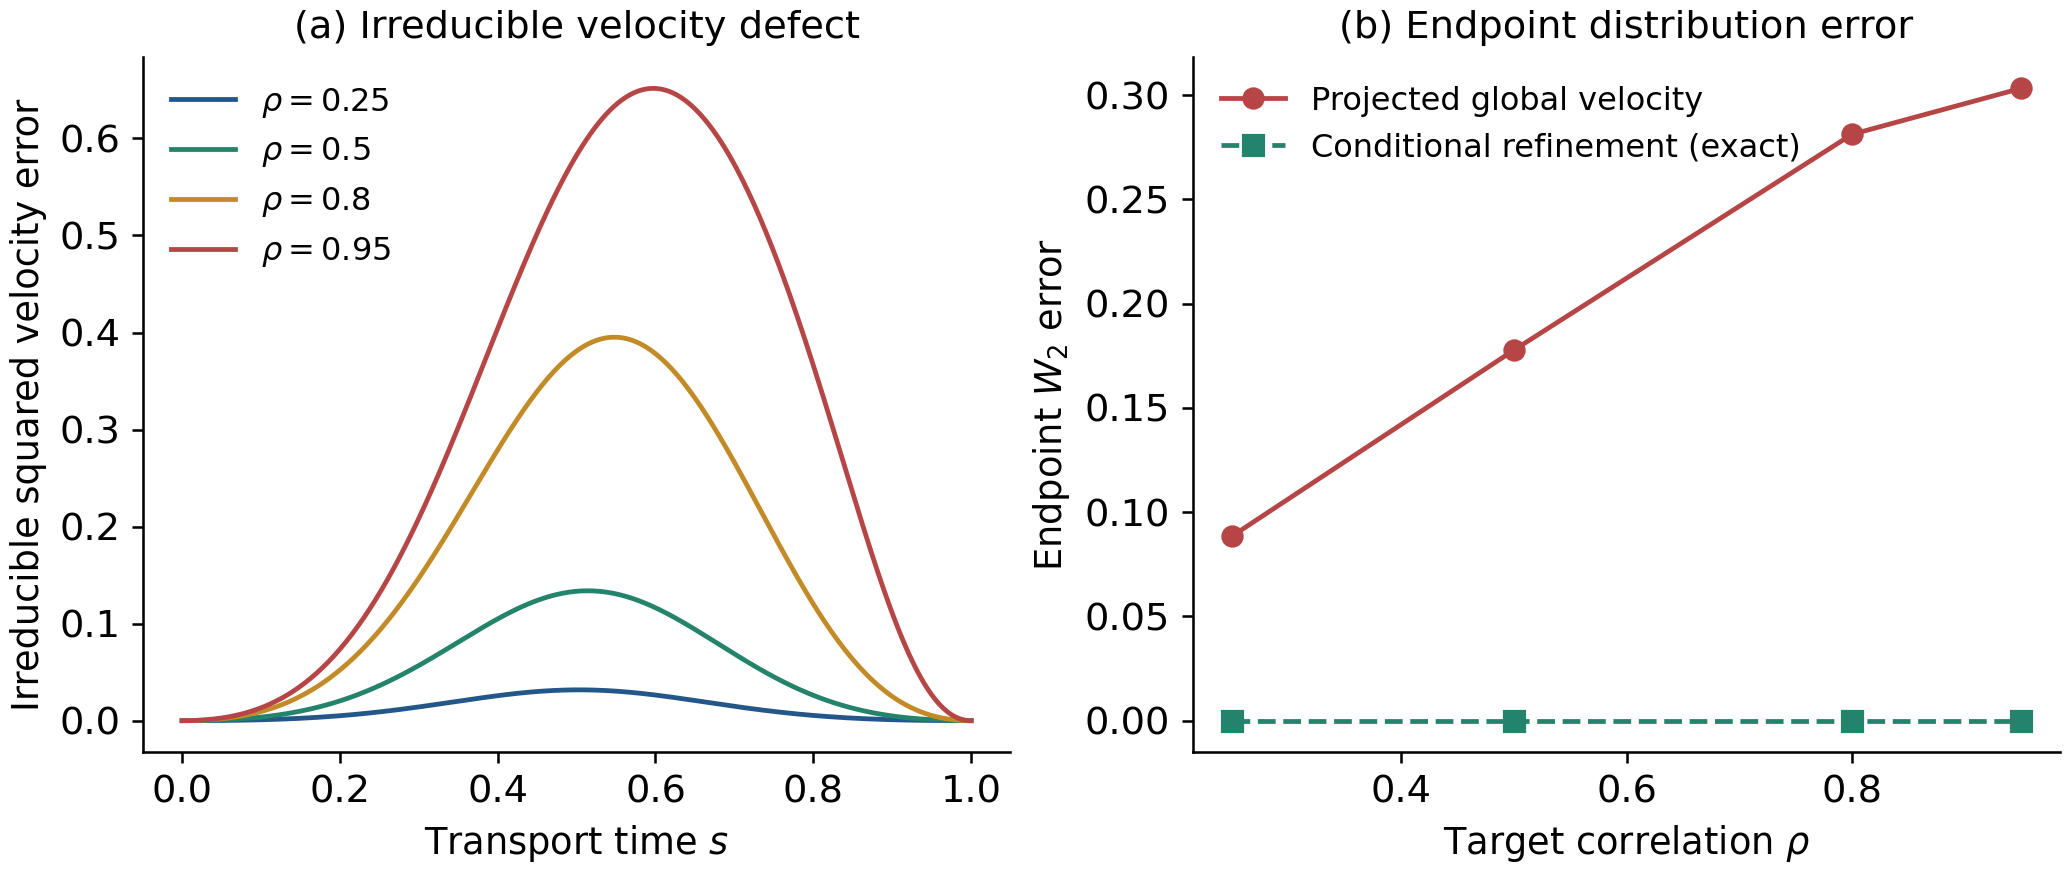
\includegraphics[width=\textwidth]{figures/bridge_obstruction.png}
\caption{Left: the exact irreducible defect $D_P(s)$ of the specified global bridge. Right: endpoint distances after integrating its unrestricted fine row and optimal coarse-only row, compared with the exact conditional refinement endpoint.}\label{fig:defect}
\end{figure}

For $\rho=0.8$, the restricted endpoint covariance is approximately
\begin{equation}
 \widehat\Sigma=
 \begin{pmatrix}
 1.000000&0.467279\\
 0.467279&0.818350
 \end{pmatrix}.
\end{equation}
It has correlation $0.516544$ and $W_2$ error $0.281233$. The observed coordinate has the correct marginal variance, but the cross-coordinate law has changed. This example makes the difference between matching projected marginals and matching a joint law directly visible.

\begin{figure}[tb]
\centering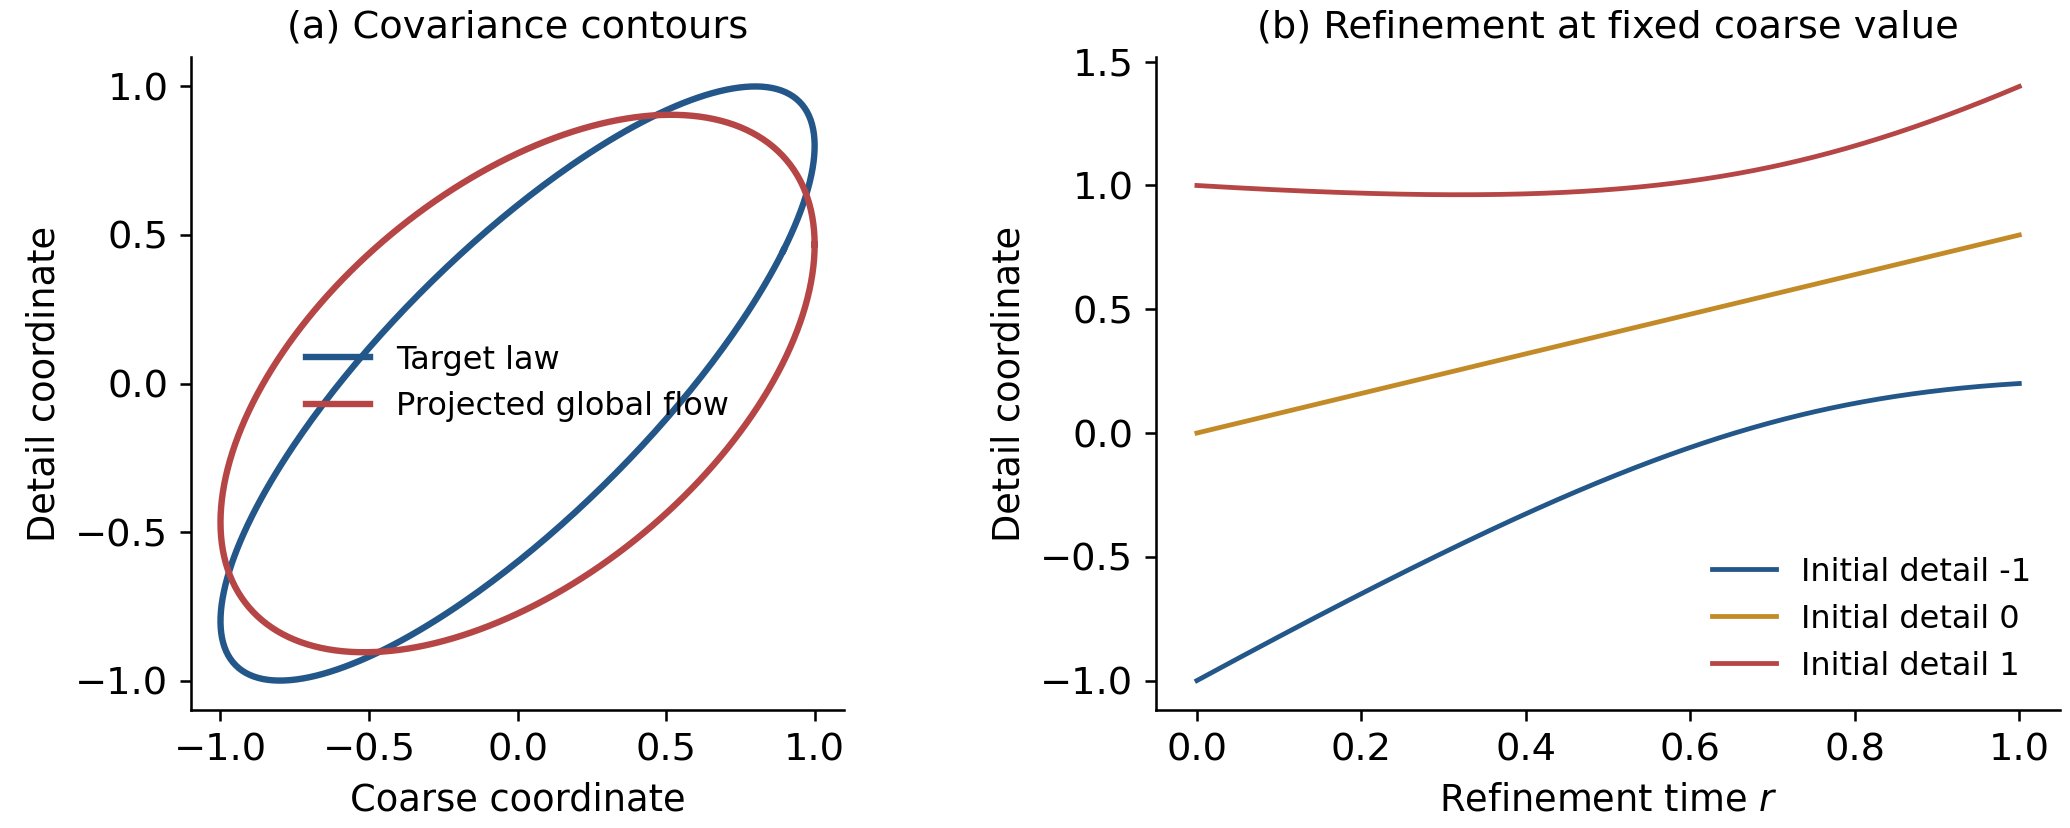
\includegraphics[width=.96\textwidth]{figures/conditional_refinement.png}
\caption{For $\rho=0.8$, the restricted global flow changes the covariance contour (left). Conditional refinement holds the sampled coarse value fixed and transports only the detail coordinate; the displayed paths use coarse value $x=1$ and three initial detail values (right).}\label{fig:conditional}
\end{figure}

\subsection{A nonlinear coherent field with an explicit accuracy certificate}
Let $H=L^2(0,1)$ with orthonormal sine basis $e_j(x)=\sqrt2\sin(j\pi x)$. Here modes are indexed by $j=1,2,\ldots$, a shift of the abstract band's initial index $0$. Define
\begin{align}\label{eq:synthetic-field}
 U_1&=\xi_1,\\
 U_j&=\frac{0.6\tanh(U_1)+0.4\tanh(U_{j-1})+\xi_j}{j},
 \qquad j\ge2,\qquad \xi_j\overset{\mathrm{iid}}\sim\mathcal N(0,1),\notag\\
 U&=\sum_{j\ge1}U_je_j.\notag
\end{align}
The conditional mean in the numerator has absolute value at most one. Since $\xi_j$ is independent of its context, $\E U_j^2\le2/j^2$ for $j\ge2$. Thus $U\in L^2(\Omega;H)$ and
\begin{equation}\label{eq:synthetic-tail}
 \tau_m^2\le2\sum_{j>m}j^{-2},\qquad m\ge1.
\end{equation}
To create an approximate conditional generator with known error, retain the first mode exactly and use
\begin{equation}\label{eq:perturbed-field}
 \widehat U_j=
 \frac{0.6\tanh(\widehat U_1)+0.4\tanh(\widehat U_{j-1})+\beta+(1+\delta)\xi_j}{j},
 \qquad \beta=0.08,\quad\delta=0.12.
\end{equation}
At the same context, the true and approximate conditional laws are Gaussian and
\begin{equation}\label{eq:synthetic-constants}
 \eps_j=\frac{\sqrt{\beta^2+\delta^2}}{j},\qquad
 L_2=\frac12,\qquad L_j\le\frac{\sqrt{0.52}}{j}\quad(j\ge3).
\end{equation}
For $j=2$, both context terms act on the same first coordinate; for later modes their gradients occupy distinct coordinates, explaining the two Lipschitz formulas. Both required square sums are finite. The theorem therefore applies to the infinite field, not just to its numerical truncation.

We use $60{,}000$ independent innovation sequences with seed $20260911$, retain a 256-mode target reference, and share each sequence between the true and approximate recursions. The coupling RMS in \Cref{tab:refinement} estimates
\begin{equation}\label{eq:coupling-mc}
 \left(\E\norm{P_{256}U-\widehat U^{(m)}}^2\right)^{1/2},
 \qquad \widehat U^{(m)}=\sum_{j=1}^m\widehat U_je_j.
\end{equation}
Its population value is an upper bound on the finite-reference $W_2$ distance. The empirical value is a sampling estimate of that bound. The last column is the deterministic full-law certificate $\sqrt{2\sum_{j>m}j^{-2}+d_m^2}$, which includes the infinite target tail.

\begin{table}[htbp]
\centering\small
\begin{tabular}{rrrr}
\toprule
Modes & Coupling RMS$^{\dagger}$ & $d_m$ & Full-law bound \\
\midrule
2 & 0.688046 & 0.072111 & 0.891666 \\
4 & 0.511363 & 0.111139 & 0.674535 \\
8 & 0.377030 & 0.133628 & 0.502872 \\
16 & 0.278531 & 0.145792 & 0.377400 \\
32 & 0.209868 & 0.152123 & 0.290989 \\
64 & 0.163959 & 0.155352 & 0.234822 \\
128 & 0.134965 & 0.156982 & 0.200518 \\
256 & 0.117721 & 0.157802 & 0.180828 \\
\bottomrule
\end{tabular}

\caption{Nonlinear refinement. $^{\dagger}$Monte Carlo estimate of the specified coupling RMS to a 256-mode target reference; it is not an optimal Wasserstein distance. $d_m$ is the exact recursively computed certificate. The last column bounds $W_2$ to the infinite target law.}\label{tab:refinement}
\end{table}
At $m=256$, the estimated coupling RMS is $0.117721$, the refinement certificate is $0.157802$, and the full-law bound is $0.180828$. The Monte Carlo standard error of the \emph{squared} coupling cost is $3.42\times10^{-5}$ at this resolution. Full values and standard errors are included in \texttt{results/metrics.json}. The separation between conditional error and tail error in \Cref{fig:certificate} reflects \eqref{eq:pythagorean-certificate}.

\begin{figure}[tb]
\centering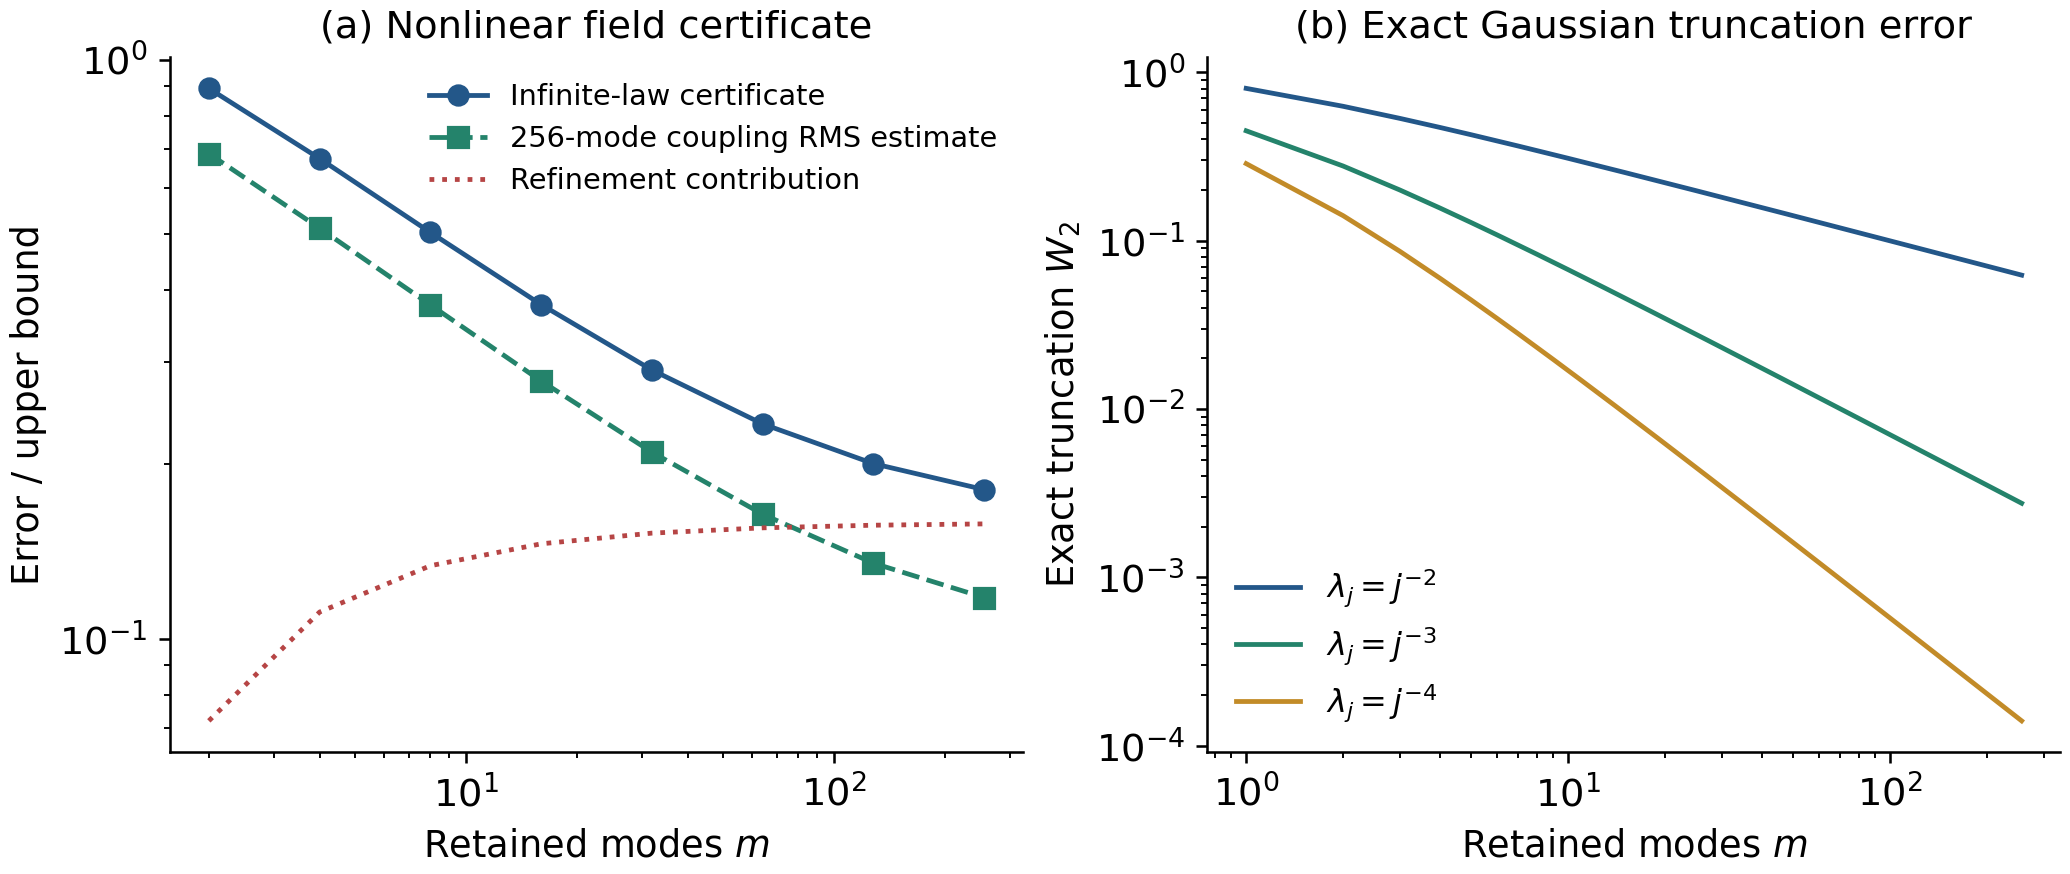
\includegraphics[width=\textwidth]{figures/refinement_certificate.png}
\caption{Left: full-law error certificates, refinement contributions, and estimated finite-reference coupling costs for the nonlinear field. Right: exact Gaussian truncation distances for three covariance spectra. These tail distances apply to generation in the retained linear subspace.}\label{fig:certificate}
\end{figure}
\begin{figure}[tb]
\centering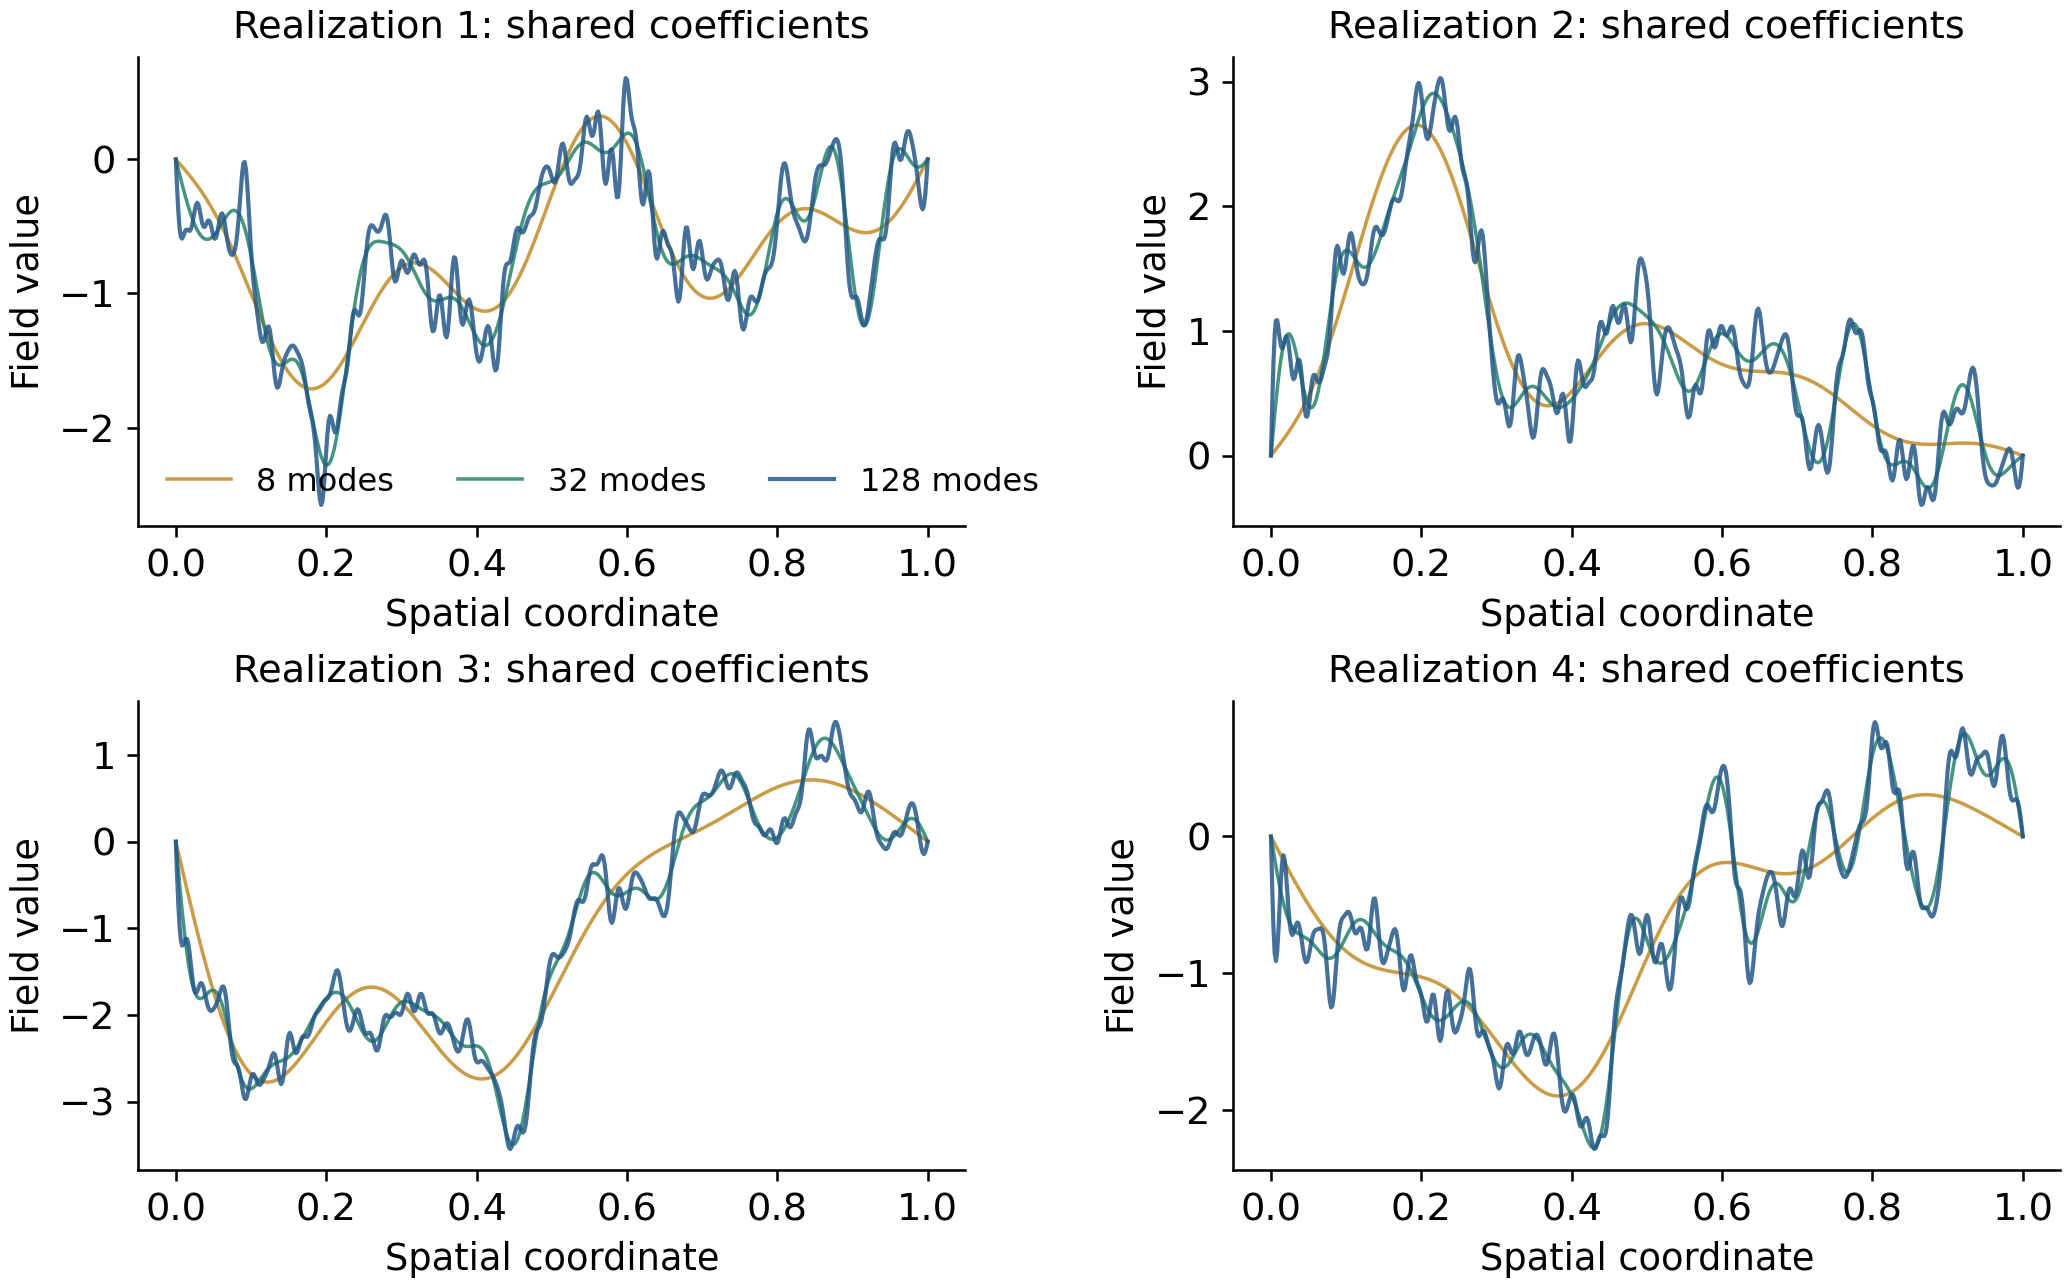
\includegraphics[width=\textwidth]{figures/coherent_fields.png}
\caption{Four realizations of the nonlinear target at 8, 32, and 128 modes using shared innovations. Lower coefficients are exactly unchanged by refinement. The curves are finite sine-series reconstructions; convergence claims in the paper concern the $L^2$ state norm.}\label{fig:fields}
\end{figure}

\subsection{A trained shared generator and simultaneous validation}\label{sec:learned-experiment}
We now learn the conditional generator for \eqref{eq:synthetic-field}. The model is \eqref{eq:neural-detail} with twelve hidden units, a softmax vector of positive output weights, and a learned positive innovation scale. It has 37 trainable parameters shared across every mode. The first mode is sampled exactly. Each hidden row is projected onto the Euclidean ball of radius $1.3$ after every update; the innovation scale is constrained to $[0.7,1.3]$.

For each of three preselected seeds, training uses 8,192 independent noisy target fields observed through mode 32. There are 1,800 Adam steps of 2,048 context/detail pairs, with learning rate $0.012$. Half the sampled pairs use mode 2 and the rest sample modes 3--32 uniformly. The objective is Gaussian conditional negative log-likelihood for the normalized coefficient $jU_j$. Conditional means are not supplied as training labels. There is no validation-based hyperparameter or seed selection.

An independent audit contains 65,536 fields through mode 256. Because the synthetic conditional mean is known, it evaluates the bounded loss in \Cref{sec:validation} with $B_j=4$. The $K=3$ candidate networks and all 255 detail modes share an overall failure probability $\delta=0.01$. The global sensitivity uses the actual learned value $K_\theta=\sum_kp_k\|a_k\|$, not a Jacobian measured at a few validation points. The values for the three runs are $0.966423$, $0.965939$, and $1.024007$; their innovation scales are $0.994923$, $1.005759$, and $0.985614$.

\begin{table}[htbp]
\centering\small
\begin{tabular}{rrrrr}
\toprule
Modes & Coupling RMS & Estimated $d_m$ & 99\% $d_m$ & 99\% full-law bound \\
\midrule
8 & 0.36176 & 0.01201 & 0.04367 & 0.48676 \\
16 & 0.25508 & 0.01283 & 0.04824 & 0.35143 \\
32 & 0.17553 & 0.01323 & 0.05065 & 0.25318 \\
64 & 0.11550 & 0.01343 & 0.05189 & 0.18357 \\
128 & 0.06724 & 0.01352 & 0.05251 & 0.13536 \\
256 & 0.00908 & 0.01357 & 0.05283 & 0.10290 \\
\bottomrule
\end{tabular}

\caption{The first preselected training seed. Coupling RMS is an empirical cost to the 256-mode target reference, and estimated $d_m$ plugs empirical conditional errors into the recurrence. The last two columns use simultaneous 99-percent conditional-error bounds; only the final column also includes the infinite target tail.}\label{tab:learned}
\end{table}

At mode 256, the empirical projected coupling RMS is respectively $0.009081$, $0.006697$, and $0.025350$. The full-law confidence bounds are $0.102899$, $0.102447$, and $0.109925$. The distinction is material: the conservative unresolved target-tail bound alone is $0.088302$, and statistical confidence also enlarges the conditional-error inputs. The standard errors of the squared coupling costs are recorded in the numerical file; they do not replace the population confidence calculation.

A separately retrained ablation removes the previous-band input while retaining the first coordinate. Its 256-mode coupling RMS is $0.105823$. Removing all mean context, while preserving the target innovation scale, gives $0.417298$. These controlled ablations isolate the value of conditional information within the stated field model. They do not rank this architecture against diffusion models or neural operators trained on other datasets.

\begin{figure}[tb]
\centering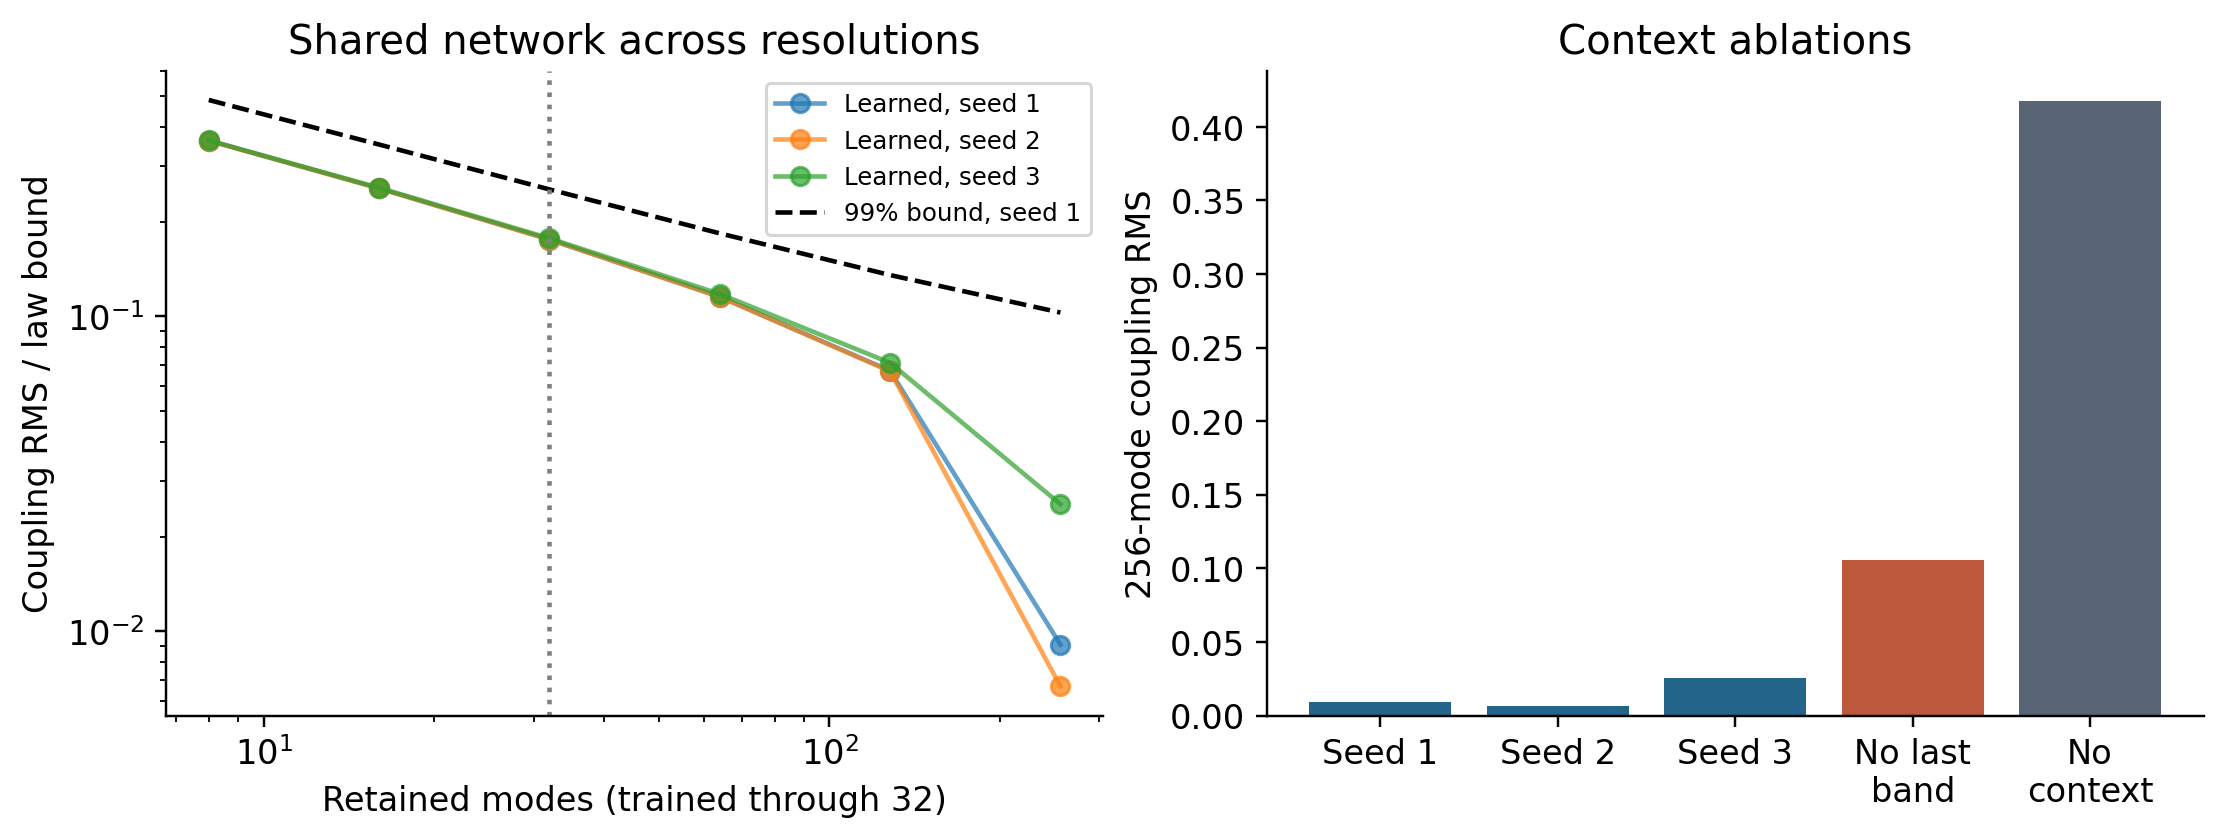
\includegraphics[width=\textwidth]{figures/learned_operator.png}
\caption{A neural model trained through 32 modes and audited through 256. The left panel distinguishes empirical finite-reference coupling costs from the first seed's full-law confidence bound. The right panel compares all three seeds with context ablations. Shared innovations reproduce every retained coefficient exactly when additional modes are requested.}\label{fig:learned}
\end{figure}

The supplied CPU float64 program records every training seed, objective, constraint, fitted parameter, bandwise fitting estimate, confidence input, and context bound. The audit uses new target fields beyond the training cutoff, so this experiment tests resolution extrapolation with known conditional laws. It does not claim that unobserved fine-scale laws can be inferred from coarse data without the structural assumptions stated in the model.

\subsection{An audit that uses observed fields without conditional-mean labels}
To test \Cref{thm:observed-audit,thm:dependency}, use the sine basis above with
\begin{equation}\label{eq:bounded-observed-field}
 U_1=X,\qquad U_j=\frac{m(X)+0.1\xi_j}{j}\quad(j\ge2),\qquad
 m(x)=0.7\tanh(0.8x)+0.1\sin(3x),
\end{equation}
where $X,\xi_2,\ldots$ are independent uniform variables on $[-1,1]$.
The first coefficient is a sufficient context for every later band. The target mean obeys $|m|\le0.8$ and $\Lip(m)\le0.86$. The target tail satisfies
$\tau_m^2\le(0.8^2+0.1^2/3)\sum_{j>m}j^{-2}$.

Three networks, with seeds $481,482,483$, each have twelve slopes and twelve softmax weights:
$f_\theta(x)=\sum_{k=1}^{12}p_k\tanh(a_kx)$.
The slopes are constrained to $[-1.3,1.3]$, giving the exact implemented sensitivity $\sum_kp_k|a_k|$. Each network trains on $16{,}384$ noisy fields through eight modes, using $1{,}200$ Adam steps and batches of $1{,}024$ randomly chosen field-mode pairs. The regression target is the observed normalized coefficient $jU_j$, not $m(X)$. Generation uses $(f_\theta(X)+0.1\xi_j)/j$. A fourth, predeclared candidate has $f=0$. All candidates share the known noise scale; learning an unspecified noise law would require a different model fit, although the distributional audit itself can compare more general scalar laws.

Two independent audit splits use seeds $7401,7402$. For budgets $n=4{,}096$, $16{,}384$, and $65{,}536$ fields per split, the feature partitions have respectively eight, twelve, and sixteen equal cells. These choices are fixed before the audit; the total failure budget $0.01$ is divided across the three budgets. Within each budget, the union bounds cover all four candidates and all 31 audited detail bands, hence every retained cutoff. Dependence between modes of one field is allowed. No cell is empty in the realized datasets; the code nevertheless implements the diameter bound for empty cells.

Both target and learned normalized details lie in $[-1.1,1.1]$. The empirical-to-model transport has a closed formula. For sorted observations $z_{(i)}$, $i=1,\ldots,n$, and a uniform model on $[c-\sigma,c+\sigma]$,
\begin{equation}\label{eq:empirical-uniform}
 W_2^2\!\left(\frac1n\sum_i\delta_{z_i},\operatorname{Unif}[c-\sigma,c+\sigma]\right)
 =\frac1n\sum_i\left[z_{(i)}-c-\sigma\left(\frac{2i-1}{n}-1\right)\right]^2
 +\frac{\sigma^2}{3n^2}.
\end{equation}
This follows by integrating the squared difference of the two quantile functions on each interval of length $1/n$. Thus the audit evaluates observed detail distributions against the learned kernel directly. It receives the support and regularity assumptions but never calls the target-mean function. Floating-point evaluation of the formula is kept distinct from a formally rounded numerical enclosure.

Because the sole parent coordinate is sampled exactly, \Cref{thm:dependency} combines the certified fitting inputs in quadrature. For seed 481 at $m=32$ and the largest budget, the generic prefix recurrence gives $0.908405$, whereas the dependency certificate gives $0.585551$. This improvement uses a proved architectural restriction, not a smaller confidence budget. Across all three trained seeds the latter bound ranges from $0.585268$ to $0.587704$. The no-context bound is $0.723932$.

\begin{table}[htbp]
\centering\small
\begin{tabular}{rrrrr}
\toprule
Fields per split & Cells & Learned bound & No-context bound & Coupling upper \\
\midrule
4,096 & 8 & 1.0304 & 1.0632 & 0.0633 \\
16,384 & 12 & 0.7653 & 0.8687 & 0.0633 \\
65,536 & 16 & 0.5856 & 0.7239 & 0.0633 \\
\bottomrule
\end{tabular}

\caption{Observed-data certification at 32 modes. The learned columns use the predeclared seed 481. Every bound includes a justified infinite target tail and belongs to the simultaneous 99\% event. The final column is a separate numerical evaluation of a specified full-law coupling, using the synthetic truth only for this diagnostic; it is not the audit input or an optimal transport distance.}\label{tab:observed-audit}
\end{table}
\begin{figure}[htbp]
\centering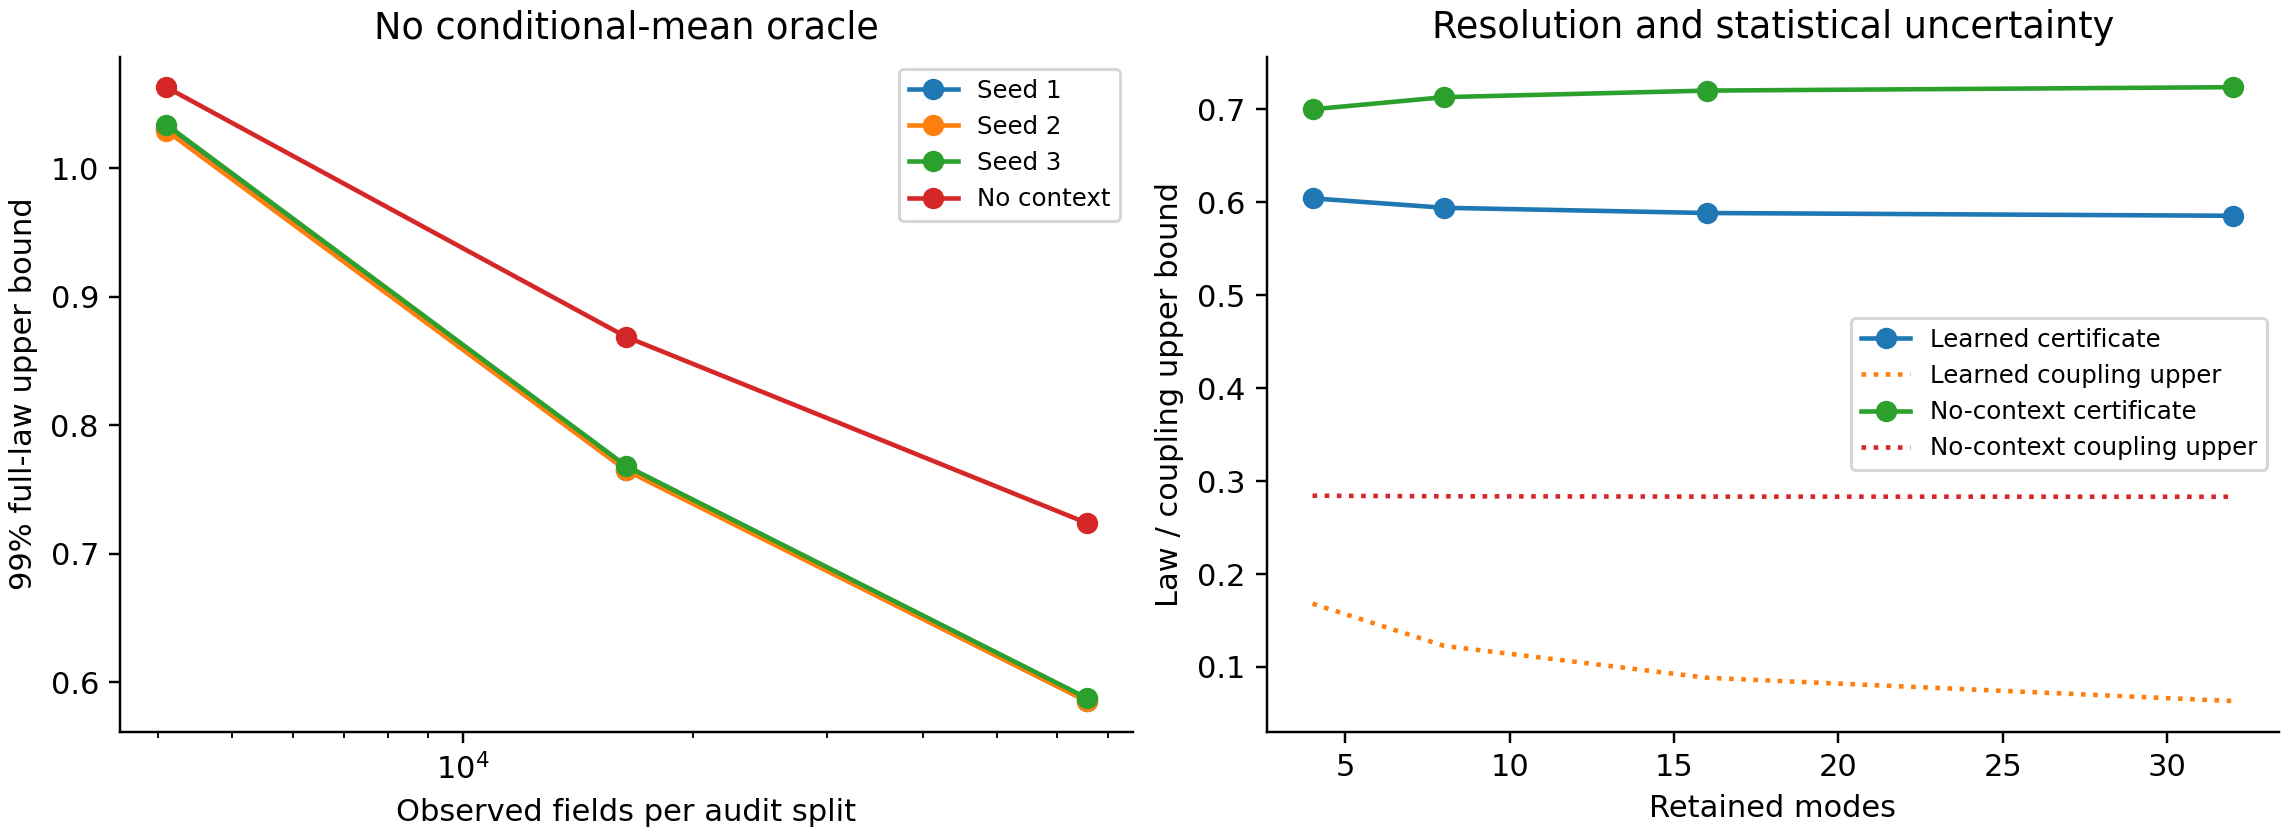
\includegraphics[width=\textwidth]{figures/observed_audit.png}
\caption{Observed-data audit with two independent splits. Left: all three trained seeds and the no-context candidate. Right: the dependence on retained resolution at the largest budget. Dotted lines evaluate a specified coupling using the known synthetic law; solid lines include statistical uncertainty and the deterministic tail envelope.}\label{fig:observed-audit}
\end{figure}

The actual conditional mean discrepancy is evaluated only in a separate truth diagnostic. Sharing $X$ and every uniform innovation makes each retained detail discrepancy $(m(X)-f_\theta(X))/j$. A 512-point Gauss--Legendre integral computes its squared mean; repeating with 1,024 points changes it by less than $10^{-15}$. For seed 481, the resulting full-law coupling upper estimate at 32 modes is $0.0633$. The much larger statistical certificate exposes the price of distribution-free cellwise estimation, the support envelope, and simultaneous coverage. The bound is informative as a guaranteed radius under the assumptions, but is not a precise estimator of the attained error. The target's analytic tail envelope also exceeds its actual tail. The code records both the generic and dependency recursions, every bandwise confidence input, cell occupancy, and all trained parameters.

\subsection{A geometry check for overlapping coordinates}
\Cref{fig:observation-geometry} evaluates the exact two-coordinate example in \Cref{sec:riesz}. The aligned discrepancy $x=y$ has squared physical-to-coordinate error ratio $1+c$, while the encoder's condition number is $\sqrt{(1+c)/(1-c)}$. The two quantities answer different questions: the former transfers a forward approximation bound, and the latter measures the worst relative instability of recovering coordinates. The plot checks the analytic formulas; it is not a fitted neural experiment.
\begin{figure}[htbp]
\centering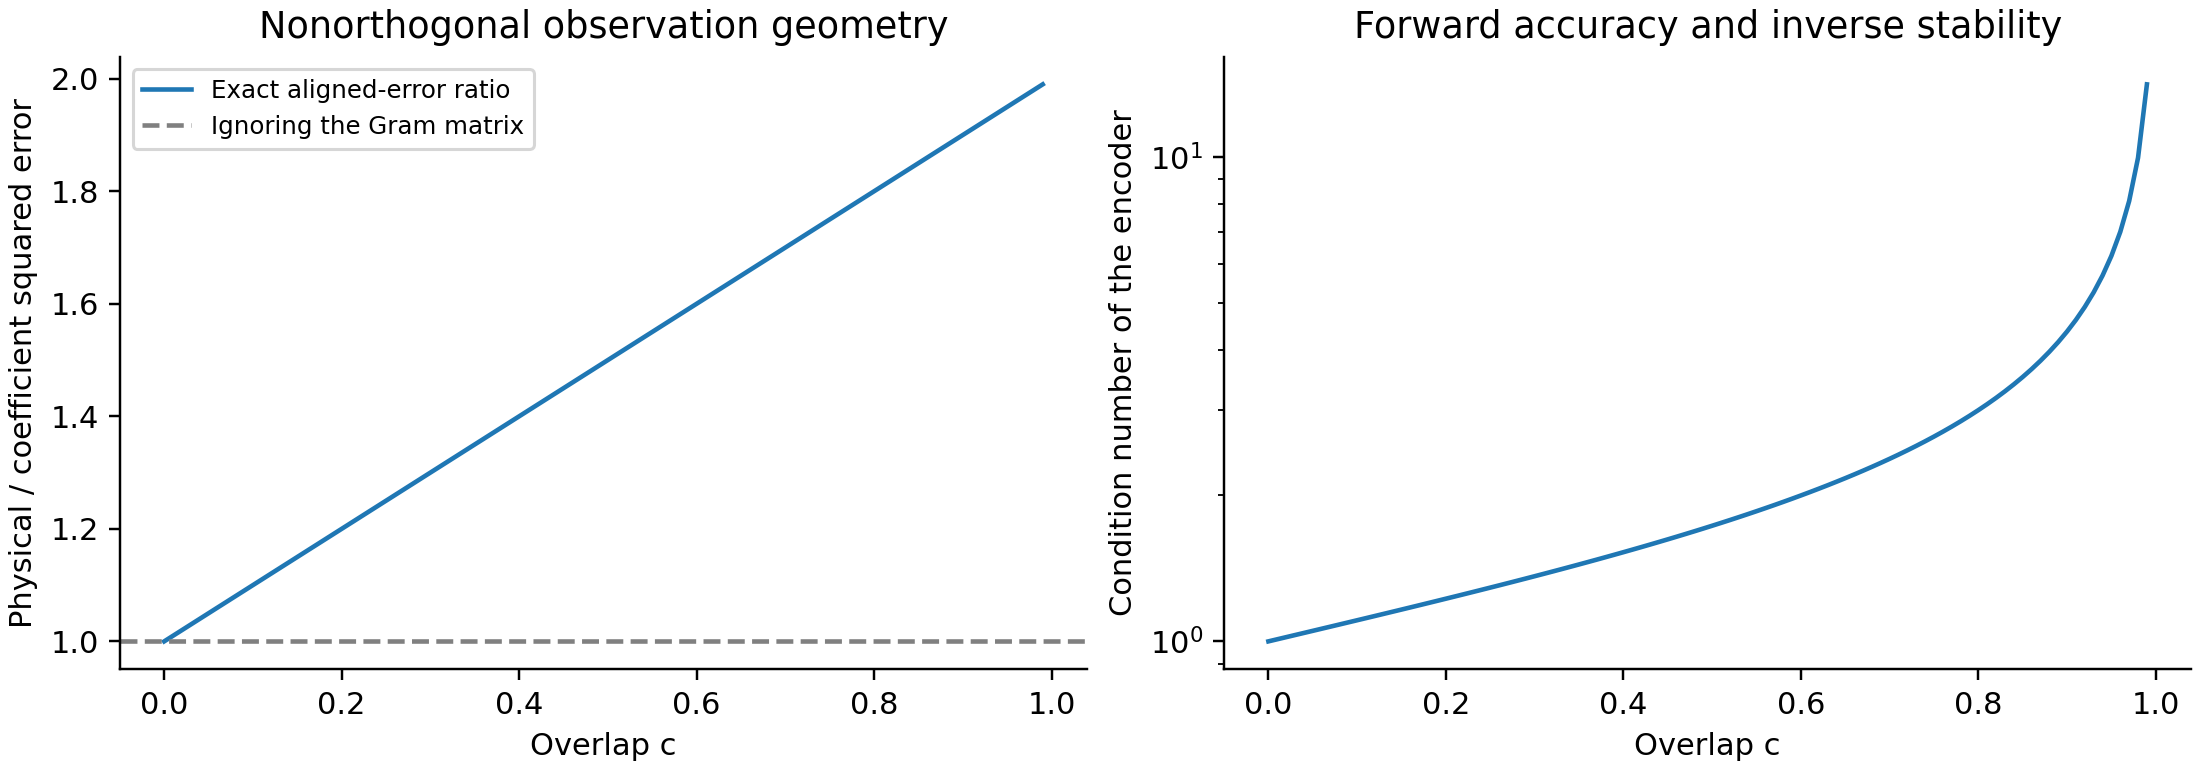
\includegraphics[width=\textwidth]{figures/observation_geometry.png}
\caption{Overlapping observation coordinates. Forward error distortion can remain bounded while the inverse representation becomes arbitrarily ill-conditioned.}\label{fig:observation-geometry}
\end{figure}


\subsection{Reproducibility and scope of numerical verification}
The script checks the orthogonal transport identity for correlated Gaussian coordinates, the sharp deterministic construction in \Cref{prop:sharpness}, the Gaussian off-diagonal defect formula, and the conditional Gaussian ODE endpoint. Their observed absolute residuals are, respectively, approximately $7.1\times10^{-15}$, zero at floating-point precision, below $2\times10^{-13}$ over the tested parameter grid, and $1.4\times10^{-12}$. These checks support implementation and arithmetic; the mathematical proofs establish the general statements.

The explicit examples isolate the bridge obstruction and sharpness mechanisms. The Gaussian trained experiment adds noisy-data fitting and a conditional-mean-based validation certificate. The bounded-field experiment uses observed conditional distributions, with no target-mean call inside its audit. Its support, sufficient context, regularity constants, and tail envelope are explicit assumptions. Both studies report all predeclared seeds. The numerical programs test implementations; the proofs establish the stated universal results.

\section{Application to market fields with hidden liquidity}\label{sec:application}
Consider a conditional model of future market fields over a price interval and a finite physical-time horizon. An illustrative state is
\begin{equation}
 U(\tau,p)=\bigl(B(\tau,p),A(\tau,p),H^b(\tau,p),H^a(\tau,p)\bigr),
\end{equation}
where $B,A$ represent displayed depth and $H^b,H^a$ represent latent reserve liquidity. Suitable scaled $L^2$ norms can treat these channels as fields. A separate event state is required when the objective includes queue identities, integer sizes, or matching-rule validity. The continuum field alone does not encode those discrete details.

The forecasting target is the full conditional path law
\begin{equation}
 c=\mathcal F_{t_0}^{\mathrm{obs}}
 \longmapsto\Law\left(U|_{[t_0,t_0+T]}\mid c\right),
\end{equation}
with information available at the forecast origin. One can choose orthogonal price aggregations or spectral detail bands inside each field channel. Generating the coarse displayed profile and then finer details gives an exactly consistent resolution family. Hidden liquidity can be added as a separate conditional component, provided its target conditional law is identified or specified by explicit modeling assumptions.

\subsection{Three consequences for model design}
First, a global flow whose displayed-depth velocity depends on latent reserve coordinates will generally have a positive autonomy defect if those coordinates are removed. Increasing the capacity of a model that still lacks the relevant state does not eliminate the defect for that prescribed flow. A posterior summary or additional predictive state can reduce it according to \Cref{prop:hierarchy-defect}.

Second, reserve liquidity inferred only from displayed depth is not automatically identifiable. If two distinct hidden-state laws produce the same observed data distribution, the two-point argument in \Cref{thm:minimax} applies. The symmetric Hilbert-space example in that theorem is mathematical; for nonnegative reserves one may instead compare two admissible nonnegative completions and obtain half their Wasserstein separation as the lower bound. Execution and replenishment data may distinguish these completions, but this requires an observation model and an identification argument.

Third, online simulation needs the physical-time condition of \Cref{thm:time}. If two full book states have the same displayed aggregate but different future displayed transition laws because their reserve states differ, an autonomous transition based on that aggregate cannot be exact for both. A filtering state such as $\pi_t$ in \eqref{eq:filter-prediction} gives a mathematically defined alternative. Auction regimes, side uncertainty, and replenishment mechanisms can be included in the hidden state without assuming that their values are observed.

The resulting model can therefore have two coupled components: a conditional field generator for spatial resolution and a state-update mechanism for physical-time events. Validity of one does not establish validity of the other. Testing should include conditional depth distributions, cross-price dependence, event-conditioned replenishment, and path functionals relevant to the intended simulator.

\subsection{Downstream observables and the chosen metric}
If $\Psi:H\to\R$ is $L_\Psi$-Lipschitz, every law certificate $W_2(\mu,\widehat\mu)\le D$ yields
\begin{equation}\label{eq:observable}
 \left|\E_\mu\Psi-\E_{\widehat\mu}\Psi\right|\le L_\Psi D.
\end{equation}
Indeed, apply the Lipschitz bound to a coupling and then Cauchy--Schwarz. Bounded linear functionals, such as weighted integrated depth, fit this condition. Threshold crossing, queue depletion indicators, and discontinuous event costs do not automatically satisfy it. For those quantities one needs a stronger state metric, boundary-mass control, or a separate distributional estimate. A small integrated field error by itself need not establish accuracy for rare events.

\section{Discussion and open questions}
The results separate four sources of difficulty: information restrictions on a prescribed bridge, fitting of conditional detail laws, sensitivity to generated contexts, and unresolved function-space energy. The autonomy defect is a conditional-variance obstruction. Conditional refinement changes the probability path and preserves previously generated coordinates. Its error propagates through an orthogonal recurrence, and summability ensures that the entire hierarchy is a probability law on the intended Hilbert space. These statements give a common language for resolution consistency without identifying it with either finite-grid weight sharing or physical-time Markov closure.

Several assumptions set the scope. The Gaussian commutation theorem uses a finite-dimensional spherical reference and a straight independent-endpoint interpolation. The sharp recurrence acts in orthogonal coefficient geometry; \Cref{thm:riesz,cor:nonlinear-decoder} transfer it through stable nonorthogonal or nonlinear representations with explicit distortion. Noninjective observation fibers remain outside that inverse-coordinate argument. For an individual model the summability conditions are sufficient; \Cref{thm:optimal-gain} proves their sharpness for uniform robustness over the full kernel class. The flow-matching corollary assumes regular exact flows and population excess losses. \Cref{thm:spectral-network,cor:validated-law} give architecture-specific energy and sensitivity guarantees and an independent validation certificate; \Cref{thm:observed-audit} adds a conditional-law audit using only observed samples and declared structural constants. None establishes universal approximation or an optimization rate. Conditional sufficiency, global regularity, and a target tail envelope must be justified in each application. Finally, projectively consistent completion determines a possible full law only after its conditional detail laws have been identified or imposed.

Three questions follow directly from the analysis. The first is statistical: can one replace the conservative cellwise audit by sharper conditional-law confidence regions, with complexity adapting to a learned sufficient context and a resolution-uniform error budget? The second is geometric: can the sharp orthogonal recurrence be extended to nonlinear observation fibers with curvature and nonunique reconstruction? The third is dynamic: which finite-dimensional summaries of the filtering distribution retain enough information to make physical-time approximation errors small while preserving useful resolution consistency? These questions require assumptions beyond the present theory, but the defect identities and certificates specify the quantities that such assumptions must control.

\subsection*{Data and code availability}
The source package includes the complete \LaTeX{} manuscript, the \texttt{plainnat} bibliography, seven PNG figures, mathematical and neural-training reproduction scripts, serialized learned parameters, generated numerical tables, and machine-readable results. The numerical examples use synthetic random variables and require no external datasets, credentials, or proprietary market feeds. The script records package versions and its random seed.

\FloatBarrier
\appendix
\section{Lean formalization and its scope}\label{sec:lean}
The accompanying Lean 4 project uses mathlib
\citep{demoura2021,mathlib2020} to check proof terms for selected universal statements. Its coverage is a strict subset of the paper: a checked real-sequence inequality, for example, still requires a probabilistic argument to supply its hypotheses.

\subsection{The refinement theorem as a formal interface}
The formal radius uses a count of completed bands:
\[
 R_0=0,\qquad
 R_{n+1}=\sqrt{R_n^2+(\eps_n+L_nR_n)^2}.
\]
Thus $R_n=d_{n-1}$ in \eqref{eq:sharp-recurrence}. The declaration
\texttt{GNO.error\_le\_radius} proves the following statement for arbitrary real sequences:
if $\eps_n,L_n,D_n\ge0$, $D_0=0$, and
\[
 D_{n+1}^2\le D_n^2+(\eps_n+L_nD_n)^2
 \quad\hbox{for every }n,
\]
then $D_n\le R_n$ for every $n$.
The proof establishes monotonicity of the nonlinear squared update and performs induction. There is no assumed axiom asserting the conclusion.

The project also proves the radius's nonnegativity and monotonicity, its exact squared recursion, its comparison with the linear majorant
\[
 A_0=0,\qquad
 A_{n+1}=(1+2L_n^2)A_n+2\eps_n^2,
\]
and the exponential estimate
\begin{equation}\label{eq:lean-exponential}
 R_n^2\le
 2\exp\left(2\sum_{j<n}L_j^2\right)\sum_{j<n}\eps_j^2.
\end{equation}
With the paper's convention $L_0=0$, this is the exponential bound in
\eqref{eq:sum-certificate}. For context-independent kernels, Lean proves the exact identity
$R_n^2=\sum_{j<n}\eps_j^2$.

The general analytic interface remains precise. The conditional-coupling proof in
\Cref{thm:certificate} supplies the squared one-step inequality for Wasserstein errors. That measure-theoretic construction is proved in the manuscript, not encoded in the Lean project. Likewise, the project does not encode disintegration, measurable selections of optimal couplings, or the Hilbert-valued infinite limit. These results are not replaced by declarations with unproved bodies.

\subsection{A finite probabilistic refinement step}
The declaration \texttt{GNO.finite\_refinement\_step} operates on an actual finite probability law $p_i\ge0$, $\sum_i p_i=1$. Let $X_i,Y_i$ be coupled old contexts and $A_i,B_i,C_i$ be the true, intermediate, and generated scalar details. From
\[
 \sum_i p_i\|X_i-Y_i\|^2\le D^2,\qquad
 \sum_i p_i(A_i-B_i)^2\le\eps^2,\qquad
 |B_i-C_i|\le L\|X_i-Y_i\|,
\]
with $D,\eps,L\ge0$, Lean proves
\begin{equation}\label{eq:lean-finite-step}
 \sum_i p_i\{\|X_i-Y_i\|^2+(A_i-C_i)^2\}
 \le D^2+(\eps+LD)^2.
\end{equation}
The proof derives weighted Cauchy--Schwarz and the finite Minkowski bound before combining the two orthogonal cost components. Thus the one-step recurrence is now connected to explicit finite joint random variables, rather than supplied only as an abstract sequence hypothesis. Construction of optimal conditional couplings and passage to general probability kernels remain written analytic arguments. The two component lemmas and this theorem are checked as finite probability statements. The additional declaration \texttt{GNO.isolated\_seed\_product} proves the exact finite product in \eqref{eq:seed-product}. The foundations project contains 35 checked declarations. In addition, \texttt{OptimalGain.lean} defines the largest eigenvalue of an arbitrary real symmetric $2\times2$ matrix, proves its characteristic identity, proves the universal quadratic upper bound, and constructs a nonzero attaining vector including diagonal degeneracies. The exact one-step energy bound used by \Cref{thm:optimal-gain} is therefore mechanized. The induction transferring attainment to the complete conditional-kernel hierarchy and the infinite-product necessity argument remain written proofs.

\subsection{Dependency, observation geometry, and statistical boundaries}
The dependency module defines a triangular radius by well-founded recursion and proves its comparison and nonnegativity for arbitrary nonnegative sensitivity coefficients. This checks the deterministic propagation in \Cref{thm:dependency}; conditional coupling supplies its probabilistic hypotheses. The observation module proves the exact two-coordinate Gram distortion, transfers a pointwise metric comparison to a normalized finite coupling cost, and proves the two-point squared-loss lower bound for a finite output law on an unobserved feature cell. It does not mechanize the probability that a cell remains unobserved.

The DKW--Massart inequality, random-cell conditioning, kernel mixture argument, Hoeffding aggregation, simultaneous confidence event, Riesz-coordinate measure correspondence, and infinite-dimensional decoder statements remain written analytic proofs. The observed-sample audit is executable Python with stated inputs; it is not represented as a Lean theorem about that program's floating-point output.

\subsection{An exact finite conditional-expectation theorem}
The regression module proves a finite conditional-expectation identity from its defining weighted averages. Let $c$ index coarse observations and $i$ index unresolved alternatives. For weights $w_{ci}$ with nonzero fiber mass
$m_c=\sum_iw_{ci}$, define
\[
 \bar v_c=\frac{\sum_iw_{ci}v_{ci}}{m_c}.
\]
For every coarse predictor $b_c$, the formal theorem establishes
\begin{align}\label{eq:lean-regression}
 \sum_{c,i}w_{ci}(v_{ci}-b_c)^2
 &=\sum_{c,i}w_{ci}(v_{ci}-\bar v_c)^2
 +\sum_cm_c(\bar v_c-b_c)^2.
\end{align}
For nonnegative weights this proves optimality of the conditional mean. After normalization, it gives the scalar finite-probability orthogonality used in \Cref{thm:defect}, for arbitrary finite index types and real values. Null fibers must be omitted.

The general Hilbert-valued conditional expectation in \Cref{thm:defect}, including time integration and almost-everywhere statements, is not formalized by \eqref{eq:lean-regression}. The geometry module separately proves the two- and three-term orthogonal squared-norm identities in an arbitrary real inner-product space.

\subsection{Gaussian and information-theoretic statements}
For the two-coordinate Gaussian example, Lean defines
$D_{\rm mid}(\rho)=2\rho^2/(4-\rho^2)$ and proves that it is nonnegative for $\rho^2<1$, strictly positive exactly when $\rho\ne0$, and equal to $8/21$ at $\rho=4/5$. The derivation of this function from Gaussian regression, the matrix commutation theorem, and the triangular Gaussian transport theorem remain written proofs.

The information module proves that in any pseudometric space, two targets at distance at least $2r$ force every common estimate to have maximum error at least $r$. It therefore checks the metric step in \Cref{thm:minimax}; the construction of the indistinguishable probability laws and their exact separation remains in the manuscript.

It also proves a general factorization equivalence. For a surjective observation map $p:X\to C$ and a map $K:X\to Y$, there exists $k:C\to Y$ with $k(p(x))=K(x)$ exactly when $K$ is constant on every fiber of $p$. The target type $Y$ may be a type of probability measures, but the formal statement does not assert measurability of $k$ or construct a measurable randomized sampler. Those are additional analytic ingredients in \Cref{thm:time}.

\begin{table}[htbp]
\centering\small
\begin{tabularx}{\textwidth}{@{}>{\raggedright\arraybackslash}p{.28\textwidth}X@{}}
\toprule
Paper result & Mechanized coverage\\
\midrule
\Cref{thm:defect} & Exact finite weighted conditional-mean loss decomposition; Hilbert orthogonal norm identities.\\
\Cref{thm:gaussian-commutation} & Positivity and exact rational value of the stated two-dimensional midpoint formula.\\
\Cref{thm:certificate} & Finite weighted joint-coupling step; nonlinear recurrence, sequence comparison, linear majorant, exponential bound, and zero-sensitivity identity.\\
\Cref{thm:optimal-gain} & Exact symmetric $2\times2$ spectral bound, characteristic identity, nonzero attainment, and one-step energy specialization.\\
\Cref{thm:dependency} & Well-founded triangular recurrence and comparison.\\
\Cref{thm:riesz,prop:unseen-cell} & Two-coordinate Gram distortion, finite coupling metric transfer, and finite two-point squared-loss obstruction.\\
\Cref{thm:minimax} & Universal two-point metric lower bound.\\
\Cref{thm:time} & Fiber-constant factorization for arbitrary types; no measurability claim.\\
\bottomrule
\end{tabularx}
\caption{Checked declarations and their analytic counterparts; coverage is partial in every row.}
\end{table}

\subsection{Rebuilding and auditing}
The toolchain is pinned to \texttt{leanprover/lean4:v4.19.0}; mathlib is pinned to its matching release and exact revision in \texttt{lake-manifest.json}. From the \texttt{lean/} directory, run
\begin{verbatim}
lake exe cache get
lake build
lake env lean Audit.lean
\end{verbatim}
Build and axiom-audit logs, a declaration-level coverage map, and source hashes are included. There are no admitted proofs, custom axioms, or unsafe proof shortcuts. Audited dependencies use only propositional extensionality, classical choice, and quotient soundness where needed. The documented executable-path compatibility adjustment changes neither Lean's kernel nor the mathematical declarations.

Formal verification does not establish empirical calibration, successful optimization, floating-point accuracy, or the physical interpretation of latent fields.

\FloatBarrier
\bigskip
\phantomsection
\addcontentsline{toc}{section}{References}
\bibliographystyle{plainnat}
\begingroup
\interlinepenalty=10000
\bibliography{references}
\endgroup
\end{document}
